%%%%%%%%%%%%%%%%%%%%%%%%%%%%%%%%%%%%%%%%%%%%%%%%%%
%%%
%%% Auteur : Stéphane Péchard - stephane.pechard@univ-nantes.fr
%%% Fichier : 1-testsub.tex - chapitre 1 : Évaluation subjective de la qualité et applications à la télévision haute définition
%%% Version : 0.1
%%% Date : 2007/06/27
%%%
%%%%%%%%%%%%%%%%%%%%%%%%%%%%%%%%%%%%%%%%%%%%%%%%%
\chapter[Évaluation subjective de la qualité visuelle et applications à la télévision haute définition]{Évaluation subjective de la qualité visuelle \\et applications à la télévision haute définition} \label{chap:evalSubj}
\opt{final}{\lettrine[lines=4]{M}{esurer la qualité visuelle}}\opt{nofinal}{Mesurer la qualité visuelle} d'une vidéo est une tâche complexe. À l'heure actuelle, il n'existe pas de meilleur évaluateur que l'\oe il humain, couplé à son cerveau. Ainsi, il est courant d'estimer de visu le résultat du traitement d'une vidéo. C'est pourquoi dans le cadre de l'évaluation d'un service de télévision, il peut être intéressant de faire intervenir des observateurs humains et de leur demander leur jugement qualitatif. Cependant, la réalisation de tels tests subjectifs soulèvent de nombreuses questions quand à leur mise en place. La variabilité du jugement humain, le contrôle des conditions d'évaluation ou encore la quantité de jugements nécessaire à une représentabilité donnée du jugement sont autant de paramètres à maitriser. Certains de ces points ont fait l'objet de travaux de recherche, allant même jusqu'à leur normalisation au niveau international.

Dans un premier temps, nous présenterons les méthodologies normalisées d'évaluation de la qualité visuelle. Nous nous interrogerons ensuite sur les aspects qui les distingue les unes des autres. Puis, nous introduirons quelques outils statistiques utiles à l'analyse des résultats fournis par les méthodologies. Enfin, nous présenterons l'état des recherches sur l'évaluation subjective de la qualité dans le contexte particulier de la télévision haute définition.


\section{À chaque méthodologie sa grandeur mesurée} \label{sec:A_chaque_methodologie_sa_grandeur_mesuree}
Le jugement humain n'étant pas stable d'un individu à l'autre, il est nécessaire d'utiliser des conditions d'expérimentations définies précisément et répétables d'un individu à l'autre et d'un environnement de test à l'autre. C'est dans ce but que l'ITU \emph{(International Telecommunication Union)} a normalisé l'ensemble des éléments intervenant dans une telle expérimentation. La figure~\ref{fig:QuiOuComment} introduit ces éléments sous forme de questions : qui mesure la qualité ? dans quelles conditions expérimentales ? suivant quelle méthodologie ? Dans ce contexte, le terme méthodologie désigne la manière dont les séquences sont évaluées pendant le test.

\begin{figure}[htbp]
  \centering
  \begin{tikzpicture}[text width=5cm]% \begin{tikzpicture}[text centered]
	\node (qui) [action, thick, minimum height=3.5cm, text width=5.1cm] {};
	\draw (0,1.2) node[text centered] {\begin{huge}\textbf{les observateurs}\end{huge}};
	\draw (0,0.6) node[anchor=north] {\begin{center}\textbf{qui ?}\end{center}\begin{itemize}\item combien ? \item quelles capacités visuelles ?\end{itemize}};

	\draw (8,0) node (ou) [action, thick, minimum height=3.5cm, text width=5cm] {};
	\draw (8,1.2) node[text centered] {\begin{huge}\textbf{l'environnement}\end{huge}};
	\draw (8,0.6) node[anchor=north] {\begin{center}\textbf{où ?}\end{center}\begin{itemize}\item quelles conditions ? \item quel affichage ?\end{itemize}};

	\draw (4,-5) node (comment) [action, thick, minimum height=4.5cm, text width=6.5cm] {};
	\draw (4,-3.5) node[text centered] {\begin{huge}\textbf{la méthodologie}\end{huge}};
	\draw (4,-5.5) node[text width=6.5cm] {\begin{center}\textbf{comment ?}\end{center}\begin{itemize}\item quelle grandeur ? \item quelle échelle ? \item quelle interface d'évaluation ? \item quelle sélection des observateurs ?\end{itemize}};

	\path[draw,thick] (qui) -- (ou) -- (comment) -- (qui);
% \end{tikzpicture}
\end{tikzpicture}
  \caption{Les différents éléments d'une évaluation subjective de qualité.}
  \label{fig:QuiOuComment}
\end{figure}

Les recommandations \ituCC{} et ITU-R BT.710-4~\cite{itu-bt710-4} sont respectivement destinées à l'évaluation de la qualité de séquences de télévision de définition standard et de télévision haute définition. La première a été très utilisée pour la TVSD, notamment par VQEG \emph{(Video Quality Experts Group)}~\cite{vqeg-frtv2}, alors que la seconde n'a pas été très développée car elle repose en grande partie sur la première. D'autres recommandations pour l'évaluation subjective de qualité existent. Par exemple, l'ITU en propose pour la qualité du son~\cite{itu-bs1284-1}, de la voix~\cite{itu-p85}, du télétexte~\cite{itu-bt812} ou du multimédia~\cite{itu-p910,itu-bt1788}. Signalons également l'approche originale de Suresh~\cite{suresh-icassp2006}. Il mesure la qualité vidéo subjective à partir de la notion de MTBF \emph{(Mean time between failure)}. Utilisé pour mesurer la fiabilité d'un produit, le MTBF est calculé comme la moyenne des temps entre deux pannes. Surech l'utilise comme une probabilité, une panne correspondant à l'apparition d'une dégradation. Les observateurs signalent chaque dégradation qu'ils perçoivent. Cette notation est binaire : soit ils perçoivent une dégradation, soit ils n'en perçoivent pas. La note de qualité finale de la séquence est calculée comme l'inverse de la probabilité de dégradation moyenne fournie par les observateurs.

Nous nous intéressons particulièrement aux différentes méthodologies d'évaluation subjective de la qualité vidéo mises à notre disposition par les recommandations internationales. Plusieurs types de grandeurs sont mesurables suivant ce que le test est sensé caractériser, ce qui implique une grande diversité de méthodologies. La figure~\ref{fig:methodoSubj} rassemble les méthodologies les plus courantes suivant la grandeur qu'elles mesurent. Dans un premier temps, nous présenterons les éléments communs à toutes les méthodologies. Puis, suivant la grandeur qu'elles mesurent, des méthodologies normalisées et utilisées pour la TVSD seront décrites.

\begin{figure}[htbp]
  \centering
  \begin{tikzpicture}[text centered,text width=2cm,scale=1.05]% \begin{tikzpicture}[text depth=1pt]
	\node (ec) at (8.2,-0.5) {};
	\node (ec2) at (8.2,-6) {};
	\node (tmp) at (10,-5) {};
	\path[draw] (ec) -| (tmp) |- (ec2);
	\node[legende,dashed,text width=4.4cm, minimum height=2cm] at (7,-0.5) {};
	\node[legende,dashed,text width=4.4cm, minimum height=1cm] at (7,-6) {};
	\node at (8.2,-0.5) {\textbf{échelle catégorielle}};
	\node at (8.2,-6) {\textbf{échelle catégorielle}};

	\node[legende,dashed,text width=4.4cm, minimum height=3.8cm] at (7,-3.5) {};
	\node at (8.2,-3.5) {\textbf{échelle continue}};

	\node[action,text width=2.5cm] (m) at (0,0)			{évaluation de\dots};
	\node[action] (g) at (3,0)				{gêne};
	\node[action] (dsis) at (6,0)			{DSIS};
	
	\node[action] (q) at (3,-1)			{qualité};
	\node[action] (acr) at (6,-1)			{ACR};
	\node[action] (sscqe) at (6,-2)		{SSCQE};
	\node[action] (dscqs) at (6,-3)		{DSCQS};
	\node[action] (samviq) at (6,-4)	{SAMVIQ};

	\node[action] (p) at (3,-5)			{préférence};
	\node[action] (sdsce) at (6,-5)		{SDSCE};
	\node[action] (p2) at (6,-6)			{SCACJ};

	\path[draw] (m) -- (g);
	\path[draw] (m) |- (q);
	\path[draw] (m) |- (p);

	\path[draw] (g) -- (dsis);
	\path[draw] (q) -- (acr);
	\path[draw] (q) |- (dscqs);
	\path[draw] (q) |- (sscqe);
	\path[draw] (q) |- (samviq);
	\path[draw] (p) -- (sdsce);
	\path[draw] (p) |- (p2);
	\path[draw] (10,-4) -- (10,-6);

% \end{tikzpicture}
\end{tikzpicture}
  \caption{Vue d'ensemble des méthodologies d'évaluation subjective de la qualité vidéo.}
  \label{fig:methodoSubj}
\end{figure}


\subsection{Conditions communes}
Bien qu'étant destinées à différentes mesures, les méthodologies normalisées que nous présentons partagent certaines conditions d'expérimentation. Ces conditions sont le panel d'observateurs, l'environnement d'observation et le déroulement global de la séance.


\subsubsection{Les observateurs}
Nous savons que pour une même séquence observée, les jugements donnés par différents individus ne sont généralement pas identiques. En d'autres termes, l'évaluation n'est pas stable d'un individu à un autre. Plusieurs facteurs en sont la cause comme l'état de fatigue, la connaissance de la séquence en question, l'expérience générale de l'observateur en évaluation de la qualité vidéo ou l'appréciation personnelle. C'est pourquoi les observateurs peuvent être regroupés en catégories. Usuellement, la première catégorisation effectuée est la séparation entre les experts et les personnes n'ayant aucune expérience de la qualité visuelle. Suivant le type de mesure effectué et l'application visée, l'âge, l'acuité visuelle et le sexe peuvent également être des critères de sélection. Par exemple, Fullerton~\cite{fullerton-josa2007} sélectionne spécifiquement des observateurs ayant une acuité visuelle comprise entre 3/100 et 4,5/10. Ainsi, il peut comparer l'impact de dégradations MPEG sur ces observateurs et sur des observateurs ayant une vision normale. Usuellement, les observateurs sont sélectionnés sans défauts visuels majeurs. Pour le déterminer, il est recommandé d'effectuer des tests visuels. Par exemple, une échelle optométrique de Monoyer~\cite{monoyer-plates} peut servir à mesurer l'acuité visuelle.

Un groupe d'évaluation idéal doit donc être constitué d'un ensemble représentatif de la population visée, selon les catégories énoncées. La recommandation \ituCC{} préconise ainsi la sélection d'au moins quinze observateurs pour obtenir une note moyenne sur une séquence. Cela peut cependant varier d'une méthodologie d'évaluation à l'autre, nous le signalerons par la suite. La note moyenne obtenue est appelée MOS \emph{(mean opinion score)}. Les observateurs doivent être non experts, c'est-à-dire qu'ils ne doivent pas être confrontés à la qualité des images ou de la vidéo dans leur activité professionnelle. Cependant, il peut être intéressant de confronter les résultats obtenus avec l'avis d'experts en qualité visuelle~\cite{svt-assesstudy}.


\subsubsection{L'environnement} \label{tests:environnement}
La mise en place d'un environnement normalisé de visualisation permet de réduire l'influence du monde extérieur sur l'observation et l'évaluation des séquences. Les facteurs couramment mesurés sont la position de l'observateur, l'ambiance générale et les caractéristiques techniques du système d'affichage.

La distance d'observation adéquate dépend du nombre de lignes de l'image. Afin de profiter au maximum de la résolution, l'idéal est de se placer à la limite de percevoir deux lignes. Le pouvoir séparateur d'une personne ayant une vision normale est en moyenne d'une minute d'arc. L'angle $\theta$ entre deux lignes tel qu'il est représenté sur la figure~\ref{fig:visualAngle}, est calculé par :
\begin{equation}
\theta = 2 \arctan\left(\frac{1}{2\times \rho\times N_L}\right)
\end{equation}
%
avec $N_L$ le nombre de lignes de l'image et $\rho$ le rapport entre la distance d'observation et la hauteur de l'écran. Ainsi, pour ne pas distinguer les 576 lignes de la TVSD, il faut se placer à une distance d'au moins :
\begin{equation}
\rho = \frac{1}{2\cdot 576\cdot \tan\left(\frac{1'}{2}\right)} = 5,96 \simeq 6 \text{ fois la hauteur de l'écran.}
\end{equation}
%
Pour les 1080 lignes de la TVHD, cette valeur est réduite à trois fois la hauteur de l'écran. Cette distance est à mesurer précisément, car elle impacte directement sur la quantité de champ visuel excité par l'affichage.% par rapport à son environnement.

\begin{figure}[htbp]
	\centering
	\begin{tikzpicture}[thick,scale=2.5]% \begin{tikzpicture}[thick,scale=2.5]
\fill[fill=white] (8,1) -- (10,0) -- (10,-2) -- (8,-1) -- cycle;
\fill[fill=blue!30] \foreach \i in {0,-0.2,-0.4,-0.6,-0.8,-1,-1.2,-1.4,-1.6,-1.8} {(8,1+\i) -- (10,\i) -- (10,\i-0.1) -- (8,1+\i-0.1) -- cycle};
\draw (8,1) -- (10,0) -- (10,-2) -- (8,-1) -- cycle;

\draw[thin] (9,-0.55) -- (7.8,-1);
\draw[fill=white] (7.8,-0.5) circle (0.5);
\draw (9,-0.5) circle (0.05);

\fill[fill=blue!30] (7.33,-.5) rectangle (8.27,-.7);
\fill[fill=blue!30] (7.31,-.5) rectangle (8.3,-.65);
\fill[fill=blue!30] (8.1,-.9) arc (-54:-126:0.5);
\fill[fill=blue!30] (7.5,-.1) rectangle (8.1,-.3);
\fill[fill=blue!30] (7.355,-.25) rectangle (8.245,-.3);
\fill[fill=blue!30] (7.383,-.25) rectangle (8.22,-.2);
\fill[fill=blue!30] (8,-.1) rectangle (8.2,-.2);
\fill[fill=blue!30] (7.41,-.18) rectangle (8,-.2);
\fill[fill=blue!30] (7.43,-.18) rectangle (8,-.15);
\fill[fill=blue!30] (7.46,-.13) rectangle (8,-.15);
\fill[fill=blue!30] (7.47,-.11) rectangle (8,-.13);

\draw[thin] (9,-0.45) -- (8.1,-0.1);
\draw (7.8,-0.5) circle (0.5);
\draw[thin] (7.49,-.1) -- (8.1,-.1);
\draw[thin] (7.35,-.3) -- (8.25,-.3);
\draw[thin] (7.3,-.5) -- (8.3,-.5);
\draw[thin] (7.35,-.7) -- (8.25,-.7);
\draw[thin] (7.49,-.9) -- (8.1,-.9);

\draw[<->] (7.8,-.6) -- (7.8,-.4) node[pos=0.5,right] {$l$};
\draw[<->] (10.1,-2) -- (10.1,0) node[pos=0.5,right] {$H=N_L\times l$};
\draw[<->] (5,-1.5) -- (8,-1.5) node[pos=0.5,above] {$O=\rho \times H$};

\draw (7.8,-.4) -- (5,-.5) -- (7.8,-.6);
% \fill[fill=blue!30] (5,-.5) arc (-10:10:5);
\draw (7,-.5) arc (0:2:2);
\draw (7,-.5) arc (0:-2:2);
\draw (7,-.5) node[right] {$\theta$};
% \end{tikzpicture}\end{tikzpicture}
	\caption{Distance d'observation $O$ en fonction du nombre de lignes de l'écran $N_L$ et du rapport $r$ avec la hauteur de l'écran $H$.}
	\label{fig:visualAngle}
\end{figure}

L'environnement ambiant agit sur l'adaptation en luminance et modifie la perception de l'image. Il doit donc lui aussi être maitrisé. Cela permet également de limiter la fatigue visuelle des observateurs. De plus, le système d'affichage utilisé lors des tests doit être exploité dans des conditions entièrement maitrisables et mesurables. Pour cela, les recommandations ITU-R BT.814~\cite{itu-bt814-1} et ITU-R BT.815~\cite{itu-bt815-1} précisent la manière de mesurer la luminance et le contraste des écrans. Elles préconisent l'utilisation de signaux spécifiques, appelés mires.


\subsubsection{Déroulement global des séances}
La structure globale d'une séance de test est commune à la plupart des méthodologies utilisées. Par contre, la procédure de présentation des séquences leur est spécifique et sera détaillée par la suite. La figure~\ref{fig:seance} donne les grandes étapes d'une séance dans l'ordre chronologique. Après la sélection d'observateurs répondant aux critères des tests visuels, une séance est précédée d'une explication sur le type de méthodologie, le système de notation, le protocole de présentation et sur tout élément que le conducteur des tests juge utile. Les conditions psychologiques dans lequel se situe l'observateur sont à la fois difficilement définissables et très influentes sur son évaluation, ce qui donne une grande importance à ses explications préliminaires. Il est également recommandé de débuter les présentations par quelques cas typiques permettant d'ancrer le jugement des observateurs. Ces présentations d'entrainement ne seront pas prises en compte dans les résultats finaux. En fin de séance, il est possible de réaliser un bilan individuel en vue de détecter d'éventuelles mauvaises appréciations.

\begin{figure}[htbp]
	\centering
	\begin{tikzpicture}[thick, text width=2cm,minimum height=1.2cm]% \begin{tikzpicture}
\draw[->] (0,0) -- (11,0);
\node[action,text width=1cm] at (1,0) {tests visuels};
\node[action] at (3,0) {explications préliminaires};
\node[action] at (5.5,0) {entrainement};
\node[action,text width=1cm] at (7.5,0) {test};
\node[action] at (9.5,0) {bilan individuel};
% \end{tikzpicture}
\end{tikzpicture}
	\caption{Étapes d'une séance d'évaluation de la qualité visuelle dans l'ordre chronologique.}
	\label{fig:seance}
\end{figure}

Une séance de test est constituée d'un nombre variable de présentation, qui correspond à l'évaluation d'une séquence. Les séquences ont en général une durée comprise entre 8 et 15 secondes afin de laisser le temps suffisant aux observateurs pour produire une note stable. Pour cela, le contenu de la séquence doit être homogène, notamment dans le cas d'une dégradation de type codage. Le cas de l'évaluation continue de plusieurs minutes et la méthodologie correspondante SSCQE \emph{(Single stimulus continuous quality evaluation)} ne sont pas considérés ici. Il est recommandé d'utiliser un ordre de présentation aléatoire, même si un observateur donné ne réalise qu'une séance. En effet, lorsqu'une séquence de bonne qualité suit une séquence de mauvaise qualité, elle va être sur-évaluée. Ces effets de contexte sont limités par un ordonnancement aléatoire des séquences. Cependant, certaines méthodologies ne permettent pas cet ordre aléatoire. Au total, une séance ne doit pas dépasser 30 à 40 minutes,  comprenant les explications, les présentations préliminaires et le bilan.


\subsection{Méthodologies de mesure de la qualité}
Les méthodologies de mesure de la qualité sont les plus nombreuses. Nous en présentons trois, que nous distinguons par le nombre de visualisation de chaque séquence.


\subsubsection{Méthodologie à stimulus unique} \label{tests:acr}
L'ACR \emph{(Absolute category rating)} consiste à porter un jugement de qualité sur des séquences présentées les unes après les autres. Il en existe deux variantes pour une visualisation unique ou triple de chaque séquence. Nous ne considérons que la première variante, plus courante. Une session de test contenant $N_S$ séquences indexées par $i\in \llbracket\text{1; }N_S\rrbracket$ consiste en la visualisation $V_i$ et l'évaluation $E_i$ de la séquence $i$. La figure~\ref{fig:acr} représente la structure d'une telle session. Chaque séquence est notée indépendamment sur une échelle de qualité à cinq catégories comme celle présentée dans le tableau~\ref{tab:echelleQualité}. Ce nombre de catégories permet une bonne discrimination sans trop de dispersion. Avec cette échelle, l'observateur ne voit que les attributs sémantiques, et non les valeurs numériques associées.

\begin{figure}[htbp]
  \centering
  % schéma de la méthode ACR

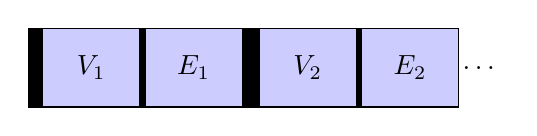
\begin{tikzpicture}
\fill[draw] (0,0) rectangle (5,1);
\path
(0.8,0.5) node [draw, fill=blue!20, minimum height=1cm, text width=1cm, text centered]    {$V_1$}
(2.1,0.5) node [draw, fill=blue!20,minimum height=1cm, text width=1cm, text centered] {$E_1$}
(3.55,0.5) node [draw, fill=blue!20, minimum height=1cm, text width=1cm, text centered]    {$V_2$}
(4.85,0.5) node [draw, fill=blue!20,minimum height=1cm, text width=1cm, text centered] {$E_2$}
(5.75,0.5) node {\dots};

\end{tikzpicture}

  \caption{Structure d'une session utilisant la méthodologie ACR. $V_i$ représente la visualisation d'une séquence et $E_i$ le vote pour cette séquence.}
  \label{fig:acr}
\end{figure}

\begin{table}[htbp]
\centering
\begin{tabular}{cc}\toprule
\strong{note}	& \strong{valeur sémantique}\\ \toprule
5				& excellent 				\\ \midrule
4				& bon 						\\ \midrule
3				& assez bon 				\\ \midrule
2				& médiocre 					\\ \midrule
1				& mauvais 					\\ \bottomrule
\end{tabular}
\caption{Échelle d'évaluation de la qualité par catégories recommandée dans la recommandation \ituCC.}
\label{tab:echelleQualité}
\end{table}

Remarquons que les séquences de référence, qu'il est recommandé d'ajouter dans la session, ne sont pas identifiées comme telles par l'observateur. Ainsi, l'ACR ne mesure pas la différence de qualité entre deux séquences, mais bien la qualité absolue de chaque séquence. Cette méthodologie est simple de mise en place et particulièrement rapide, permettant de juger un grand nombre de séquences par session. Par exemple, dans le cadre du Test Plan Multimedia~\cite{vqeg-MMtestplan}, VQEG évalue 166 séquences de huit secondes en une session de 35 minutes environ. La contrepartie de ce rendement est la précision, nécessitant un nombre d'observateurs important. Ainsi, VQEG préconise d'utiliser un panel d'au moins 24 observateurs.


\subsubsection{Méthodologie à double stimuli} \label{tests:dscqs}
Une autre manière de faire est de présenter explicitement la référence à l'observateur, et de lui demander de noter la version altérée en gardant en mémoire son appréciation de la référence. Ceci est particulièrement indiqué lorsque la vidéo de référence est disponible. Appelée DSCQS \emph{(Double Stimuli Continuous Quality Scale)}, cette méthodologie présente aléatoirement la version dégradée et la version de référence. Dans l'exemple de la figure ~\ref{fig:dscqs}, la vidéo dégradée est placée en premier. La méthodologie prévoit la possibilité de répéter plusieurs fois la présentation avant la notation. Cela permet d'affiner l'évaluation mais allonge d'autant la durée de la séance. Il est courant ici de considérer le DMOS \emph{(differential mean opinion score)}, définie comme la différence entre le MOS de la référence et le MOS de la séquence dégradée. Cette méthodologie est donc adaptée à la mesure de fidélité, c'est-à-dire de l'écart d'un signal à une référence dans l'espace de qualité.

\begin{figure}[htbp]
  \centering
  % schéma de la variante 2 de la méthode DSIS

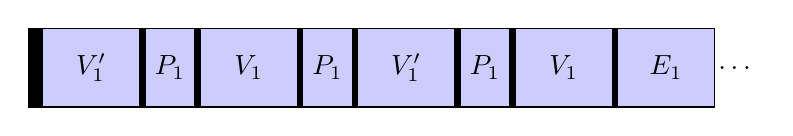
\begin{tikzpicture}
\fill[draw] (0,0) rectangle (8.5,1);
\path
(0.8,0.5) node [draw, fill=blue!20, minimum height=1cm, text width=1cm, text centered]    {$V'_1$}
(1.8,0.5) node [draw, fill=blue!20, minimum height=1cm, text width=0.4cm, text centered]    {$P_1$}
(2.8,0.5) node [draw, fill=blue!20, minimum height=1cm, text width=1cm, text centered]    {$V_1$}
(3.8,0.5) node [draw, fill=blue!20, minimum height=1cm, text width=0.4cm, text centered]    {$P_1$}
(4.8,0.5) node [draw, fill=blue!20, minimum height=1cm, text width=1cm, text centered]    {$V'_1$}
(5.8,0.5) node [draw, fill=blue!20, minimum height=1cm, text width=0.4cm, text centered]    {$P_1$}
(6.8,0.5) node [draw, fill=blue!20, minimum height=1cm, text width=1cm, text centered]    {$V_1$}
(8.1,0.5) node [draw, fill=blue!20, minimum height=1cm, text width=1cm, text centered]    {$E_1$}
(9,0.5) node {\dots};

\end{tikzpicture}
  \caption{Structure de présentation de la DSCQS~\cite{itu-bt500-11}. $V_i$ représente la visualisation de la séquence de référence, $V'_i$ de la séquence dégradée, $P_i$ la pause et $E_i$ le vote pour cette séquence.}
  \label{fig:dscqs}
\end{figure}

Contrairement à l'ACR, la DSCQS utilise une échelle d'évaluation continue, présentée sur la figure~\ref{fig:echelleQualitéContinue}. Cette échelle comporte 100 notes différentes, allant de 1 à 100 par pas de 1. Les observateurs attribuent à chaque séquence une valeur numérique placée sur un segment de droite. Celui-ci est séparé en zones, étiquetées par les mêmes attributs sémantiques que l'échelle par catégories de l'ACR. Ces attributs permettent de donner une consistance à l'ensemble de l'échelle, afin d'éviter les différences d'utilisation. Ce type d'échelle permet ainsi d'affiner le jugement au sein d'une catégorie.

\begin{figure}[htbp]
  \centering
  \begin{tikzpicture}[scale=0.95]% schéma d'une échelle de qualité pour les méthodes par comparaison avec échelle d'évaluation continue

% \begin{tikzpicture}
  \draw (0,0) -- (0,5)
  node at (-1,4.5) {excellent}
  node at (-1,3.5) {bon}
  node at (-1,2.5) {assez bon}
  node at (-1,1.5) {médiocre}
  node at (-1,0.5) {mauvais};
  \draw (-0.1,5) -- (0.1,5) node[right]{100};
  \draw (-0.1,4) -- (0.1,4);
  \draw (-0.1,3) -- (0.1,3);
  \draw (-0.1,2) -- (0.1,2);
  \draw (-0.1,1) -- (0.1,1);
  \draw (-0.1,0) -- (0.1,0) node[right]{0};
% \end{tikzpicture}
\end{tikzpicture}
  \caption{Échelle continue d'évaluation de la qualité.}
  \label{fig:echelleQualitéContinue}
\end{figure}


\subsubsection{Méthodologie à stimuli multiples} \label{tests:samviq}
Cette méthodologie est la plus récente. Bien que les autres soient répandues et utilisées par plusieurs laboratoires, l'EBU ne les considère pas suffisamment stables pour évaluer les applications comme la vidéo sur Internet ou sur appareil mobile. C'est pourquoi elle a proposé cette méthodologie d'évaluation, également applicable aux systèmes de télévision. Cette méthodologie présente l'intérêt majeur de pouvoir discriminer des qualités proches les unes des autres~\cite{blin-vpqm2006}.

SAMVIQ \emph{(Subjective assessment methodology for video quality)}~\cite{ebu-samviq} est une méthodologie d'évaluation à stimuli multiples et à échelle de qualité continue. Elle utilise à la fois une référence cachée et une référence explicite, c'est-à-dire clairement identifiée par l'environnement de test. De plus, elle propose une visualisation à accès aléatoire, c'est-à-dire que l'observateur choisit l'ordre dans lequel il visionne les séquences et peut suivre son propre rythme pour l'évaluation, la modification des notes et la répétition des séquences. De ce fait, SAMVIQ ne peut pas être utilisée avec plusieurs observateurs simultanément, contrairement à ACR ou DSQCS. Le nombre de visualisation pour chaque séquence n'est pas limité, c'est la dernière note attribuée qui est enregistrée. Par contre, toutes les séquences doivent être visualisées au moins une fois. Plusieurs contenus, chacun ayant subi plusieurs traitements sont évaluables par session. Ainsi, alors que l'ACR permet l'évaluation de 166 séquences de 10 secondes par session d'environ 35 minutes, SAMVIQ est limitée à 48. Cependant, le fait de pouvoir affiner son jugement en regardant plusieurs fois les mêmes séquences permet d'augmenter la précision de la mesure, et donc de diminuer le nombre d'observateurs à quinze. SAMVIQ transforme le jugement de plusieurs observateurs ayant vu une fois une séquence en jugement de moins d'observateurs l'ayant vu plusieurs fois. %Sa précision vient donc de l'échange de dispersion inter-observateurs par de la dispersion intra-observateur.

SAMVIQ utilise deux ancrages sur l'échelle de qualité, l'un de haut niveau, l'autre de bas niveau. Cela permet d'exploiter l'échelle de qualité au maximum et de stabiliser la notation, facilitant les comparaisons de résultats entre laboratoires et entre tests. La séquence de référence est utilisée comme ancrage de haut niveau : c'est la référence explicite. L'ancrage de bas niveau peut être défini soit par une version codée à bas débit, soit par une version synthétique produite par ajout de flou et diminution de la fréquence d'image. L'EBU préfère cette dernière manière d'opérer car la version obtenue est plus stable et aisément reproductible dans différents laboratoires. En plus des différentes versions traitées à tester, une présentation doit donc obligatoirement contenir la version de référence explicite, la version de référence cachée et la version d'ancrage de bas niveau. Typiquement, une session est composée de quatre présentations de cinq à douze séquences.

Historiquement, les notions d'accès aléatoire et d'ancrage viennent d'études sur l'audio réalisées par l'EBU. La méthodologie d'évaluation de la qualité sonore MUSHRA \emph{(Multiple stimuli with hidden reference and anchor)} utilise ce procédé~\cite{kozamernik-mushra,itu-bs1534}. Les auditeurs écoutent des séquences audio au rythme et dans l’ordre de leur choix et leur attribuent une note. Parmi ces séquences figurent des séquences de référence cachées de très bonne et de très mauvaise qualité. L'EBU estime que ce type d'approche apporte une meilleure estimation par individu de la qualité pour différentes versions d'une vidéo. En effet, le fait d'avoir à noter un ensemble de traitements lors d'une même présentation assure le maintien d'une bonne relation d'ordre de notation pour chaque individu et améliore la cohérence globale des tests. Le défaut pratique de SAMVIQ est qu'elle ne permet qu'un nombre limité d'évaluation pour un même contenu~\cite{huynhthu-vpqm2007}. Concernant le résultat de l'évaluation, le réalisme de l'accès aléatoire est discutable, dans la mesure où il repose sur une multi-visualisation non représentative de l'usage réel.


\subsection{Méthodologie de mesure de la gêne ressentie}
Cette méthodologie se nomme DSIS \emph{(double stimulus impairment scale)}. Deux variantes sont possibles, en présentant les séquences soit une seule fois, soit deux fois. La structure de la seconde est présentée sur la figure~\ref{fig:dsis}. L'échelle de notation utilisée est ici une échelle de dégradation comme celle présentée dans le tableau~\ref{tab:echelleDégradations}. Chaque attribut sémantique associé à une catégorie correspond à une appréciation de la gêne ressentie par l'observateur. Bien que, comme pour la DSCQS, le résultat issu de ce test soit un MOS, la différence sémantique est importante, et se traduit par une tâche différente pour les observateurs. L'intérêt est une plus grande stabilité de jugement pour un observateur donné.

\begin{figure}[htbp]
	\centering
	% schéma de la variante 2 de la méthode DSIS

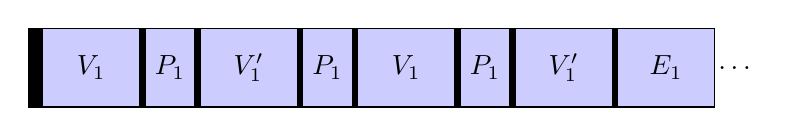
\begin{tikzpicture}
\fill[draw] (0,0) rectangle (8.5,1);
\path
(0.8,0.5) node [draw, fill=blue!20, minimum height=1cm, text width=1cm, text centered]    {$V_1$}
(1.8,0.5) node [draw, fill=blue!20, minimum height=1cm, text width=0.4cm, text centered]    {$P_1$}
(2.8,0.5) node [draw, fill=blue!20, minimum height=1cm, text width=1cm, text centered]    {$V'_1$}
(3.8,0.5) node [draw, fill=blue!20, minimum height=1cm, text width=0.4cm, text centered]    {$P_1$}
(4.8,0.5) node [draw, fill=blue!20, minimum height=1cm, text width=1cm, text centered]    {$V_1$}
(5.8,0.5) node [draw, fill=blue!20, minimum height=1cm, text width=0.4cm, text centered]    {$P_1$}
(6.8,0.5) node [draw, fill=blue!20, minimum height=1cm, text width=1cm, text centered]    {$V'_1$}
(8.1,0.5) node [draw, fill=blue!20, minimum height=1cm, text width=1cm, text centered]    {$E_1$}
(9,0.5) node {\dots};

\end{tikzpicture}
	\caption{Structures de la variante 2 de la DSIS. $V_i$ représente la visualisation de la séquence de référence, $V'_i$ de la séquence dégradée, $P_i$ la pause et $E_i$ le vote pour cette séquence.}
  \label{fig:dsis}
\end{figure}

\begin{table}[htbp]
\centering
\begin{tabular}{ccc}\toprule
\strong{note}	& \strong{valeur sémantique}\\ \toprule
5				& imperceptibles \\ \midrule
4				& perceptibles mais non gênantes \\ \midrule
3				& légèrement gênantes \\ \midrule
2				& gênantes \\ \midrule
1				& très gênantes \\ \bottomrule
\end{tabular}
\caption{Échelle d'évaluation des distorsions par catégories~\cite{itu-bt500-11}.}
\label{tab:echelleDégradations}
\end{table}


\subsection{Méthodologies de mesure de la préférence entre différentes versions} \label{sec:Méthodes_de_mesure_de_la_préférence_entre_différentes_versions}
Ces méthodologies travaillent par comparaison, en situant une vidéo par rapport à une autre dans l'espace de qualité. Deux séquences sont présentées à l'observateur qui doit mesurer la relation entre les deux en termes de qualité visuelle. Pour cela, deux échelles d'évaluation sont utilisables.% : une échelle par catégorie ou une échelle continue.


\subsubsection{Méthodologie avec échelle d'évaluation par catégorie} \label{ssec:Méthode_avec_échelle_dévaluation_par_catégorie}
La méthodologie SCACJ \emph{(Stimulus comparison adjectival categorical judgement)} utilise une telle échelle. Les observateurs attribuent la relation entre les séquences à une catégorie définie sémantiquement. Un exemple d'échelle est présenté dans le tableau~\ref{tab:echelleCompCategories}. %Ici, les termes employés n'ont pas de connotation qualitative tel que \emph{bon} ou \emph{mauvais}.
Il existe plusieurs ensembles de catégories, suivant ce que le test cherche à caractériser. Il est possible de mesurer la présence de différences perceptibles, leur direction ou bien à la fois l'étendu et la direction, comme dans l'exemple présenté dans le tableau~\ref{tab:echelleCompCategories}. La manière d'analyser les résultats dépend à la fois du jugement effectué et de l'information recherchée.

\begin{table}[htbp]
\centering
\begin{tabular}{cc}
\toprule
\strong{note} & \strong{valeur sémantique} \\ \toprule
-3 & Beaucoup moins bon \\ \midrule
-2 & Moins bon \\ \midrule
-1 & Légèrement moins bon \\ \midrule
0 & Identique \\ \midrule
+1 & Légèrement mieux \\ \midrule
+2 & Mieux \\ \midrule
+3 & Beaucoup mieux \\ \bottomrule
\end{tabular}
\caption{Exemple d'échelle catégorielle d'évaluation de la qualité~\cite{itu-bt500-11}.}
\label{tab:echelleCompCategories}
\end{table}


\subsubsection{Méthodologie avec échelle d'évaluation continue}
La méthodologie SDSCE \emph{(Simultaneous double stimulus for continuous evaluation)} utilise ce type d'échelle. Les observateurs attribuent à chaque relation une valeur numérique placée sur un segment de droite. Celui-ci peut être séparé en zones, chacune étant étiquetée d'un adjectif qualificatif. Ces adjectifs peuvent caractériser une qualité comme ceux présentés sur la figure~\ref{fig:echellecontinueComparaison} ou bien une différence (de identique à différent) qu'il s'agit de quantifier.

\begin{figure}[htbp]
	\centering
	% schéma d'une échelle de qualité pour les méthodes par comparaison avec échelle d'évaluation continue

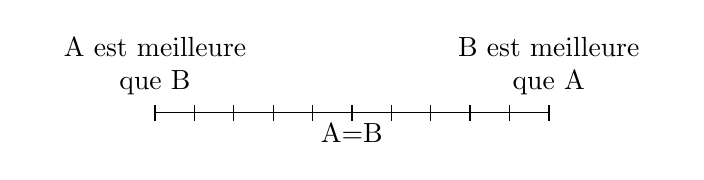
\begin{tikzpicture}
  \draw (0,0) -- (5,0);
  \draw[thick] (5,-0.1) -- (5,0.1)  node[above, text width=3cm, text centered] {B est meilleure que A};
  \draw (4.5,-0.1) -- (4.5,0.1);
  \draw (4,-0.1) -- (4,0.1);
  \draw (3.5,-0.1) -- (3.5,0.1);
  \draw (3,-0.1) -- (3,0.1);
  \draw[thick] (2.5,-0.1) -- (2.5,0.1) node [below=0.1cm] {A=B};
  \draw (2,-0.1) -- (2,0.1);
  \draw (1.5,-0.1) -- (1.5,0.1);
  \draw (1,-0.1) -- (1,0.1);
  \draw (0.5,-0.1) -- (0.5,0.1);
  \draw[thick] (0,-0.1) -- (0,0.1) node[above, text width=3cm, text centered] {A est meilleure que B};
\end{tikzpicture}
	\caption{Exemple d'échelle continue d'évaluation de la qualité~\cite{itu-bt500-11}.}
	\label{fig:echellecontinueComparaison}
\end{figure}


\subsection{Conclusion}
Le tableau~\ref{tab:comparaisonméthodologies} récapitule les caractéristiques intéressantes des principales méthodologies proposées par les normes internationales. Dédiées à la mesure d'une grandeur donnée, elles permettent d'analyser la perception par l'observateur moyen de la qualité, la gêne ou encore la préférence entre séquences vidéo. Chacune a ses avantages et ses inconvénients, rendant le choix dépendant de nombreux facteurs. Nous avons ainsi commencé à aborder l'équilibre entre la précision de la mesure et le nombre d'observateurs requis. Détaillons maintenant les différents points de comparaison entres les méthodologies.

\begin{table}[htbp]
\centering
\begin{tabular}{cccccc}\toprule
\strong{paramètre}			& \strong{ACR} 	& \strong{DSIS}	& \strong{DSCQS}	& \strong{SAMVIQ}	& \strong{SDSCE} \\ \toprule
évaluation de					& qualité				& gêne					& qualité					& qualité					& préférence\\\midrule
référence explicite			& 							& \texttimes			& \texttimes				& \texttimes				& \texttimes\\\midrule
référence cachée 			& \texttimes			&							& 								& \texttimes				& \\\midrule
ancre haute						& \texttimes			& 							& \texttimes				& référence cachée	& \\\midrule
ancre basse						& \texttimes			& 							& \texttimes				& \texttimes				& \\\midrule
échelle								& catégorielle		& catégorielle		& continue				& continue				& continue \\\midrule
nombre de visualisation	& 1						& 1 ou 2				& 2							& multiple					& 1 \\\midrule
nombre d'observateurs 	& \multirow{2}{1.3cm}{1 ou plus} 	& \multirow{2}{1.3cm}{1 ou plus} & \multirow{2}{1.3cm}{1 ou plus}	& \multirow{2}{1cm}{1} & \multirow{2}{1.3cm}{1 ou plus} \\
simultanés & & & & &\\\bottomrule
\end{tabular}
\caption{Exemple d'échelle catégorielle d'évaluation de la qualité~\cite{itu-bt500-11}.}
\label{tab:comparaisonméthodologies}
\end{table}



\section{Comparaison des méthodologies} \label{sec:ComparaisonDesMethodes}
Malgré l'importance et le cout des évaluations subjectives de qualité vidéo, il existe peu d'études comparatives sur les méthodologies existantes. Elles ont pourtant chacune des caractéristiques différentes. Les principales différences que nous pouvons identifiées sont :
\begin{itemize}
\item le type d'échelle utilisée ;
\item le nombre de visualisation de chaque séquence ;
\item la présence ou non de la référence explicite.
\end{itemize}
%
Quelques études ont été menées pour mettre en lumière ces différences. Nous les décrivons ci-après.


\subsection{Type d'échelle}
Van den Ende~\cite{ende-ei2007} compare le DSIS et le DSCQS dans le cadre de l'évaluation de séquences de TVSD ayant subis différents codages MPEG-2. Seize observateurs sont séparés en deux groupes de même taille. Afin d'éviter les effets de contexte liés à l'ordre d'utilisation des deux méthodologies, un groupe donné utilise d'abord le DSCQS puis le DSIS, l'autre groupe faisant l'inverse. Les notes de chaque méthodologie sont transformées en Z-scores afin d'être comparés. Les remarques des observateurs indiquent qu'ils considèrent le DSIS plus aisé à utiliser. Cela peut s'expliquer par le fait qu'il n'y ait qu'une séquence à noter, relativement à une autre, alors que le DSCQS requiert deux notations, dont celui de la référence. De plus, le DSIS ne laisse pas la possibilité de variation autour des termes qu'il utilise. Si les observateurs considèrent l'échelle suffisante pour discriminer les différentes séquences, le DSIS est alors particulièrement adapté. Les coefficients de corrélation inter-groupes sont le plus souvent élevées : entre 0,853 et 0,996, sachant que la valeur immédiatement supérieure à 0,853 est 0,921. Cependant, l'un des contenus testés dans l'une des configurations pose problème. Les corrélations sont comprises entre 0,364 et 0,782 sans que les auteurs ne soient en mesure d'identifier clairement l'origine de cette chute.

Dans son étude sur les effets de contexte, Corriveau~\cite{corriveau-subjScales} compare le DSCQS, le DSIS et le SDSCE sur des séquences au format PAL. Les résultats issus du DSIS sont convertis en DMOS sur une échelle $[\text{0 ; }\text{100}]$. Les trois méthodologies fournissent des résultats cohérents et similaires, mais les auteurs remarquent deux effets. Le premier est que les méthodologies n'utilisent pas les mêmes gammes de qualité. Ainsi, les DMOS issus du DSCQS ne dépassent pas 70, alors qu'ils atteignent 95 avec les deux autres. L'auteur pense que les observateurs ont tendance à éviter les notes extrêmes allant de 0 à 25 et de 85 à 100 avec le DSCQS. En revanche, en présence de très bonnes ou très mauvaises qualités, l'observateur n'a pas de variations possibles autour des notes extrêmes du DSIS. C'est en fait le cas sur toute l'échelle en raison de la quantification de l'échelle, mais c'est surtout visible aux extrémités. Or, bien que l'échelle soit continue, le même effet apparait avec le SDSCE. L'auteur l'explique par le fait que le DMOS doit être jugé sur la moitié de l'échelle seulement, de l'absence de préférence à la préférence maximale. Le second effet est que les méthodologies se révèlent différemment sensibles aux effets de contexte. Les résultats ne révèlent aucun effet contextuel pour le DSCQS, des effets contextuels modérés pour le SDSCE et des effets contextuels importants pour la DSIS. Sans tenter d'expliquer l'origine de ce constat, l'auteur conclut que le DSCQS est la meilleure méthodologie à utiliser afin de minimiser les effets contextuels.

Une explication pourrait être que le DSCQS requérant les évaluations des deux séquences qu'il présente, il force l'observateur à plus d'attention, notamment sur la référence. Dans le DSIS, seule la version dégradée est notée. L'ancrage, bien qu'existant, peut être moins bien ressenti par l'observateur, expliquant une influence plus forte des qualités des séquences voisines.


\subsection{Nombre de visualisation}
Ce nombre varie de un au nombre désiré par l'observateur. Ainsi, avec SAMVIQ, l'observateur peut visualiser une séquence autant de fois que nécessaire. Le jugement peut alors se construire sur l'apprentissage de la séquence et de ses dégradations, ce que ne permet pas l'ACR ou le DSIS.

Huynh-Thu~\cite{huynhthu-sip2005} compare DSCQS et ACR dans un contexte de codage bas débit de séquences au format QCIF \emph{(Quarter Common Intermediate Format)}. Afin de comparer les deux ensemble de données, les MOS issus du DSCQS sont quantifiés linéairement pour passer de l'échelle $[\text{0 ; }\text{100}]$ à l'échelle $[\text{1 ; }\text{5}]$ de l'ACR. Le même nombre d'observateurs est utilisé pour les deux tests, ce qui a tendance à produire des intervalles de confiance plus grands pour l'ACR. Le coefficient de corrélation entre les MOS obtenus sur les deux ensembles est très élevé : 0,975. Cela signifie que les deux méthodologies permettent d'évaluer les séquences de manière similaire. Ici, bien que le DSCQS permette de visualiser deux fois chaque séquence, cela ne semble pas créer de différences significatives entre les résultats des deux ensembles.

Brotherton~\cite{brotherton-ieice2006} compare SAMVIQ et ACR dans ce même contexte de codage à bas débit, mais avec des séquences au format CIF. La comparaison des données issues des deux méthodologies fournit une bonne corrélation de l'ordre de 0,94. L'auteur remarque une différence significative d'évaluation pour une dégradation de type réduction du nombre d'images par seconde. SAMVIQ est plus critique dans ce cas, fournissant des notes significativement inférieures à l'ACR. Cela s'expliquerait par la possibilité de répétition de la séquence, qui permettrait de mettre en évidence les dégradations et leur importance. SAMVIQ serait ainsi plus fiable pour des erreurs occasionnelles comme le gel d'image. La répétition permet d'affiner le jugement, même s'il devient alors plus artificiel, car basé sur un usage non conventionnel de la visualisation des images en télévision.

Il est regrettable que les auteurs ne fournissent que le coefficient de corrélation comme indicateurs de performances. En effet, celui-ci ne renseigne pas sur la cohérence ni sur la précision de la relation entre les ensembles de notes. Néanmoins, ces études ont montré l'impact du nombre de visualisations sur l'apprentissage des séquences à évaluer. Il ne semble pas y avoir de différences significatives entre une et deux visualisations. Par contre, les multiples visualisations proposées par SAMVIQ semblent créer une différence dans certaines conditions. Il reste cependant à clairement identifier ces conditions.


\subsection{Présence de la référence explicite}
La vidéo de référence n'est pas toujours identifiée comme telle par l'observateur. C'est la différence entre référence explicite et référence cachée. Cette dernière sert à valider la relation d'ordre des qualités et la cohérence des réponses. Nous ne nous intéressons ici qu'à la référence explicite. Sa présence modifie la tâche de l'observateur. Sans référence, il doit juger de la qualité dans l'absolu, sans point de repère. En présence de la référence, l'observateur doit créer une relation entre les deux qualités et noter son importance. C'est la notion de fidélité qui est en jeu. La fidélité est la capacité à s'approcher d'un idéal, représenté par la référence.

Lee~\cite{lee-ie2006} compare le DSCQS avec l'ACR et le SSCQE. Cette dernière diffère du DSCQS par deux aspects. Tout d'abord, le nombre de visualisations de chaque séquence est réduit à un. Ensuite, l'observateur visualise une unique séquence, résultat de la concaténation de séquences de dix secondes. Les notes de qualité sont relevées toutes les demi-secondes. Pour l'ACR et le DSCQS, des séquences de huit secondes issues de cette longue séquence sont évaluées. La note obtenue est comparée à la moyenne des notes issues de la SSCQE. L'auteur obtient de très fortes corrélations entre les notes issues des méthodologies ACR et DSCQS, comprises entre 0,92 et 0,96 et obtenues avec respectivement 20 et 19 observateurs. Cela confirme les résultats obtenus par Huynh-Thu~\cite{huynhthu-sip2005}. La présence de la référence modifie donc peu le jugement absolu des observateurs, ce qui tend à montrer que ce jugement est relativement indépendant du contenu. Par contre, les corrélations entre SSCQE et DSCQS sont comprises entre 0,810 et 0,846 avec respectivement 23 et 18 observateurs. Ces performances semblent montrer que le SSCQE ne permet pas une notation aussi fiable que le DSCQS. Cela peut provenir soit de la fatigue engendrée par la longueur de la séquence à évaluer, soit des effets de contexte liés aux transitions entre les séquences, soit d'un mauvais alignement temporel des notations continues avec la note du DSCQS. Ce dernier point n'est cependant pas détaillé par les auteurs. Au final, la multiplicité des raisons pouvant expliquer la chute de performance empêchent de clairement identifier l'impact de la présence de la référence explicite dans la comparaison entre SSCQE et DSCQS.


\subsection{Conclusion}
Nous avons identifié trois principaux points de comparaison entre les méthodologies. Chacun a été mis en relief par des expérimentations présentées dans la littérature.
%
% Les différences d'usage de l'échelle de notation entre DSCQS et DSIS a montré l'impact du type d'échelle. La comparaison entre ACR et SAMVIQ a laissé apparaitre des conditions où le nombre de visualisations des séquences auraient un impact sur leur notation. Cependant, les conditions précises provoquant ces différences restent encore à identifier. Enfin, la bonne corrélation entre DSCQS et ACR laisse penser que la présence de la référence explicite dans la méthodologie d'évaluation a peu d'impact sur le résultat.
Cependant, certaines zones d'ombre demeurent. En effet, ces études se contentent de relever les différences sans identifier clairement les conditions qui les provoquent et celles qui n'ont pas d'influence. De plus, alors que la précision d'une évaluation semble provenir du nombre de visualisation, aucune étude n'a défini les limites du compromis entre la précision et le nombre d'observateurs nécessaire pour l'atteindre. Remarquons enfin qu'aucune de ces expérimentations ne s'est intéressée à l'impact du format d'image.


\section{Analyse des évaluations}
Au cours d'une évaluation subjective de qualité, une quantité importante de données est récoltée. Il convient alors d'effectuer quelques vérifications avant de traduire ces données en résultats. Ainsi, la cohérence inter-observateurs est couramment évaluée. Suite à cette vérification, les évaluations de certains observateurs peuvent être rejetées. Cette étape peut donc s'avérer critique dans l'obtention des résultats d'une méthodologie puisque celle-ci nécessite un nombre minimal d'observateurs retenus. De plus, les tests pouvant faire partie de vastes campagnes de mesures effectuées par plusieurs laboratoires, il est nécessaire de d'évaluer l'homogénéité des différents résultats avant de les agréger en un unique ensemble. Une fois l'intégrité des résultats vérifiée, des outils de synthèse sont utilisés afin de résumer les tendances mesurées. Des outils statistiques simples sont souvent utilisés, mais suivant le type de test effectué, des outils plus originaux peuvent être intéressants. Nous présentons ici des algorithmes de vérification des observateurs, une méthode d'évaluation de mesures inter-laboratoires et des outils de synthèse des résultats.


\subsection{Vérification des observateurs}
Un observateur peut commettre une erreur en évaluant une séquence, ou même sur l'ensemble d'une session. Une analyse précise doit permettre d'éliminer ces erreurs. C'est pourquoi des critères de rejet des observateurs sont élaborés. Deux méthodes sont présentées ici. La première est de l'ITU~\cite{itu-bt500-11} et utilise le test dit du $\beta_2$. La seconde est de l'EBU~\cite{ebu-samviq} et utilise les coefficients de corrélation. Malgré l'aspect sensible de cette vérification, il n'existe pas d'étude concernant la comparaison ou la validation de ces méthodes.


\subsubsection{Méthode par le test du \texorpdfstring{$\beta_2$}{beta2}} \label{sssec:rejet-itu}
La méthode commence par s'assurer que la distribution des $N_n$ notes est normale grâce au test du $\beta_2$, c'est-à-dire le moment d'ordre quatre divisé par le carré du moment d'ordre deux :
\begin{equation}
\left(\beta_2\right)_{jkl} = \frac{\dfrac{1}{N_n} \sum\limits_{i=1}^{N_n} \left(\text{MOS}_{ijkl} - \overline{\text{MOS}}_{jkl}\right)^4}{\left(\dfrac{1}{N_n} \sum\limits_{i=1}^{N_n} \left(\text{MOS}_{ijkl} - \overline{\text{MOS}}_{jkl}\right)^2\right)^2}
\end{equation}
%
avec $\text{MOS}_{ijkl}$ le MOS donné par l'observateur $i$ à la condition $j$ de la séquence $k$ lors de la répétition $l$ de la visualisation et $\text{MOS}_{jkl}$ la moyenne de ces MOS sur les observateurs. S'il est compris entre deux et quatre, la distribution est considérée comme normale. Puis pour chaque observateur $i$, les paramètres $\omega_i$ et $\Omega_i$ initialisés à zéro énumèrent le nombre de valeurs s'éloignant significativement de la moyenne.

Si $2 \leqslant \left(\beta_2\right)_{jkl} \leqslant 4$,
\begin{equation*}\begin{array}{cc}
\text{si}\quad \text{MOS}_{ijkl} \geqslant \overline{\text{MOS}}_{jkl} + 2\cdot\sigma_{jkl},\quad \text{alors}\quad \omega_i = \omega_i + 1\, ; \\
\text{si}\quad \text{MOS}_{ijkl} < \overline{\text{MOS}}_{jkl} - 2\cdot\sigma_{jkl},\quad \text{alors}\quad \Omega_i = \Omega_i + 1.
\end{array}
\end{equation*}

Sinon,
\begin{equation*}\begin{array}{cc}
\text{si}\quad \text{MOS}_{ijkl} \geqslant \overline{\text{MOS}}_{jkl} + \sqrt{20}\cdot\sigma_{jkl},\quad \text{alors}\quad \omega_i = \omega_i + 1\, ; \\
\text{si}\quad \text{MOS}_{ijkl} < \overline{\text{MOS}}_{jkl} - \sqrt{20}\cdot\sigma_{jkl},\quad \text{alors}\quad \Omega_i = \Omega_i + 1.
\end{array}
\end{equation*}

Avec $N_j$ le nombre de conditions (incluant la référence), $N_k$ le nombre de séquences et $N_l$ le nombre de répétitions, le test final est :
\begin{equation*}
\text{si}\quad \frac{\omega_i + \Omega_i}{N_j \cdot N_k \cdot N_l} > 0.05\quad\text{et}\quad\left|\frac{\omega_i - \Omega_i}{\omega_i + \Omega_i}\right| < 0.3%\quad \text{alors l'observateur } i \text{ est rejeté}.
\end{equation*}
%
alors l'observateur $i$ est rejeté.

Le premier terme traduit la quantité de valeurs significativement éloignées de la moyenne. Si cette quantité est trop grande, le second terme permet de conserver les observateurs qui s'éloignent toujours dans le même sens. La méthode tolère ainsi les écarts, sauf si ils dénotent une inconstance dans la notation. Ainsi, les observateurs peuvent surévaluer ou sous-évaluer leurs notations, dans la mesure où ils en conservent la cohérence. Cet algorithme est utilisé par les méthodologies ACR, DSCQS et DSIS.


\subsubsection{Méthode par comparaison de coefficients de corrélation} \label{sssec:rejet-samviq}
La méthode SAMVIQ de l'EBU présentée en~\ref{tests:samviq} propose son propre algorithme d'évaluation des observateurs. Ce critère de rejet vérifie la consistance sur une session des notes d'un observateur par rapport à la moyenne de tous les observateurs. Il utilise pour cela le coefficient de corrélation linéaire de Pearson~\cite{pearson-rslpt} entre $x$ et $y$ :
\begin{equation}
r_p(x,y) = \frac{\left(\sum\limits_{i=1}^{N_c} x_i \cdot y_i\right) - \dfrac{\left(\sum\limits_{i=1}^{N_c} x_i\right)\left(\sum\limits_{i=1}^{N_c} y_i\right)}{{N_c}}}{\sqrt{\left(\sum\limits_{i=1}^{N_c} x_i^2 - \dfrac{\left(\sum\limits_{i=1}^{N_c} x_i\right)^2}{{N_c}} \right)\left(\sum\limits_{i=1}^{N_c} y_i^2 - \dfrac{\left(\sum\limits_{i=1}^{N_c} y_i\right)^2}{{N_c}} \right)}}
\label{eq:pearson}
\end{equation}
%
avec $i$ la condition de test, $x_i$ le score moyen de tous les observateurs sur la condition $i$, $y_i$ le score d'un observateur sur la condition $i$ et ${N_c}$ le nombre de conditions. Il utilise également le coefficient de corrélation de rang de Spearman~\cite{spearman-ajp} entre ces mêmes $x$ et $y$ :
\begin{equation}
r_s(x,y) = 1 - \dfrac{6\times\sum\limits_{i=1}^{N_c} \left[r(x_i) - r(y_i)\right]^2}{N_c^3 - N_c}
\label{eq:spearman}
\end{equation}
%
avec $r(X)$ le rang de l'élément $X$. L'algorithme de rejet évalue ensuite l'écart entre le minimum de ces deux coefficients pour l'observateur testé et pour l'ensemble des observateurs. Si le minimum d'un observateur est au-dessus d'un certain seuil, celui-ci est rejeté.

Une variante de ce critère est utilisée par VQEG~\cite{vqeg-MMtestplan}. La différence est que celui-ci compare deux coefficients de corrélation de Pearson entre le MOS et la note de l'observateur à évaluer. Le premier $r_p^\text{1}$ est calculé l'ensemble des séquences ayant été notées par les observateurs. Le second $r_p^\text{2}$ est calculé par traitement en moyennant toutes les notes de ce traitement. Le critère de rejet consiste ensuite à exclure un observateur si $r_p^\text{1}$ et $r_p^\text{2}$ sont chacun sous un seuil donné. Ces seuils sont paramétrables, ce qui permet d'adapter la tolérance d'acceptation des observateurs. Cette liberté pose cependant la question du compromis entre la quantité d'observateurs rejetés qui doit être minimale et la qualité finale de l'évaluation qui nécessite le rejet d'observateurs non cohérents. L'utilité de l'analyse par traitement est qu'un observateur peut avoir une préférence pour un certain contenu, tout en ayant tout de même voté de manière consistante sur l'ensemble des séquences. Cette analyse permet de moyenner l'effet des préférences individuelles et de vérifier la consistance des évaluations selon les traitements.

Outre le fait que ce type d'analyse peut ne pas rejeter tous les observateurs non cohérents, il existe également un risque de spécialisation. En effet, un observateur est rejeté par rapport à une moyenne, supposée représenté le comportement moyen face à l'évaluation. Cependant, il peut arriver qu'un sous-ensemble des observateurs ait un comportement différent mais commun. S'il est important, ce sous-ensemble va alors être considéré comme le comportement moyen et les observateurs s'en écartant seront rejetés. Cela peut se présenter, par exemple, si l'échantillon d'observateurs n'est pas représentatif.


\subsection{Agrégation d'évaluation inter-laboratoires}
Dans le but de vérifier si plusieurs laboratoires procurent des données ayant le même comportement pour la même évaluation de qualité et le même nombre d'observateurs, l'EBU utilise le test Wilcoxon~\cite{wilcoxon-bb}. Il consiste à vérifier si deux échantillons peuvent être issus de la même loi en étudiant comment les valeurs de chacun se situent parmi les statistiques de l'échantillon global. Pour cela, l'algorithme calcule les différences entre toutes les notes de qualités mesurées. Puis, il ordonne les valeurs absolues des différences dans l'ordre croissant et calcule les sommes des rangs des différences positives et négatives. Le minimum $S_w$ de ces deux sommes est alors comparé aux valeurs de $\xi$ fournit dans le tableau~\ref{tab:wilcoxon}. Si il est inférieur à $\xi$, alors les données sont considérées équivalentes, à 5\% près. La valeur de $\xi$ dépend du nombre d'observateurs. Plus ils sont nombreux et plus l'algorithme est tolérant sur l'écart entre $S_w$ et $\xi$.

\begin{table}[htbp]
	\centering
	\begin{tabular}[c]{cccccccccccccc}\toprule
		\strong{nombre d'observateurs} & 6 & 7 & 8 & 9 & 10 & 11 & 12 & 13 & 14 & 15 & 16 & 17 & 18 \\ \midrule
		$\xi$ & 0 & 2 & 3 & 5 & 8 & 10 & 13 & 17 & 21 & 25 & 29 & 34 & 40 \\ \bottomrule
	\end{tabular}
	\caption{Données du test Wilcoxon.}
	\label{tab:wilcoxon}
\end{table}

Cet algorithme permet de savoir s'il est possible d'agréger des données issues de tests effectués de la même manière, mais dans des lieux différents. Ce contexte inter-laboratoire est notamment courant pour VQEG dont les tests du Multimedia Test Plan~\cite{vqeg-MMtestplan} sont réalisés dans sept laboratoires différents.


\subsection{Outils statistiques de synthèse}
La première mesure utile est le score moyen $\overline{u}_{jk}$ sur les observateurs, c'est-à-dire le MOS de chaque présentation :
\begin{equation}
\overline{u}_{jk} = \frac{1}{N_i} \sum\limits^{N_i}_{i=1} u_{ijk}
\end{equation}
%
avec $N_i$ le nombre d'observateurs et $u_{ijk}$ le score de l'observateur $i$ pour la condition $j$ et la vidéo $k$. La moyenne $\overline{u}_j$ pour chaque condition et $\overline{u}_k$ pour chaque vidéo peuvent également être utilisées. Dans le but d'évaluer la fiabilité des résultats, il est recommandé d'accompagner chaque MOS de son intervalle de confiance. L'intervalle de confiance à 95\% est utilisé en pratique : $[\overline{u}_{jk} - \delta_{jk}\, ;\, \overline{u}_{jk} + \delta_{jk}]$ avec :
\begin{equation}
\delta_{jk} = 1,96\cdot \dfrac{\sqrt{\sum\limits_{i=1}^{N_i} \dfrac{(\overline{u}_{jk} - u_{ijk})}{N_i-1}}}{\sqrt{N_i}}.
\end{equation}


\subsection{Modèle de comparaison par paires}
L'évaluation préférentielle telle qu'elle est effectuée avec les méthodologies SDSCE et SCACJ s'apparente à une comparaison par paires de toutes les séquences évaluées. Dans ce cas particulier, le problème est de traduire l'ensemble des évaluations binaires des observateurs en une note de qualité et en un intervalle de confiance pour chaque séquence de l'ensemble.

Pour cela, Reibman~\cite{reibman-vpqm2006} utilise le modèle de comparaison par paires de Bradley--Terry~\cite{bradley-biometrika}. Dans ce modèle, la qualité relative entre deux séquences $i$ et $j$ vaut $Q_i - Q_j = \log \pi_i - \log \pi_j$ avec $\frac{\pi_i}{\pi_i+\pi_j}$ la probabilité que la séquence $i$ soit préférée à la séquence $j$, $\sum_i \pi_i = 1$ et $\forall i, \pi_i \geqslant 0$. La fonction de vraisemblance est alors :
\begin{equation}
L = \frac{\prod\limits_i \pi_{i}^{a_i}}{\prod\limits_{i<j} (\pi_i + \pi_j)^{N_{\textit{ij}}}}
\end{equation}
%
avec $N_{\textit{ij}}$ le nombre de fois où chaque paire est comparée et $a_i$ le nombre total de fois où la séquence $i$ est préférée aux autres séquences. Le maximum de cette fonction correspond alors aux qualités produisant les évaluations subjectives de plus grande probabilité. L'estimation du maximum de vraisemblance de $\pi_i$ est :
\begin{equation}
p_i = \frac{a_i}{\sum\limits_{j, j\neq j} \frac{N_{\textit{ij}}}{p_i + p_j}}
\end{equation}
%
avec $i \in [1;N_s]$ et $N_s$ le nombre de séquences comparées. Ces équations peuvent être résolues de manière itérative. Des formules pour celles-ci sont données par Dykstra~\cite{dykstra-biometrics}.% à partir de données approchées

À titre d'exemple, détaillons comment Reibman utilise ce modèle dans le cadre de l'évaluation de qualité d'images reconstruites à une résolution donnée à partir de plusieurs images de résolutions inférieures. Son algorithme de « super-résolution » est sensé atténuer les dégradations introduites par ce type de reconstruction. Entre 22 et 33 observateurs ont évalué un ensemble de seize conditions de test, issues de trois images de référence et de plusieurs valeurs d'un paramètre de l'algorithme. Une comparaison par paires exhaustive nécessiterait donc $C_{16}^2=$ 120 comparaisons pour chacun des observateurs. En pratique, Reibman réduit ce nombre afin que les séances de test ne soient pas trop longues. La figure~\ref{fig:reibmanVpqm2006} présente le type de résultat obtenu. La figure~\ref{reibman1} représente l'estimation de la qualité relative par le maximum de vraisemblance en fonction du paramètre de l'algorithme pour les trois images. La figure~\ref{reibman1} est l'équivalent pour une seule des trois images. Les qualités sont relatives car c'est ce que fournit le modèle de Bradley--Terry. Pour l'affichage, la moyenne des qualités vaut zéro.

\begin{figure}[htbp]
	\centering
	\subfloat[Pour les trois images\label{reibman1}.]{\begin{tikzpicture}[scale=0.853]% \begin{tikzpicture}[scale=0.85]
\node at (-3.5,2.75) {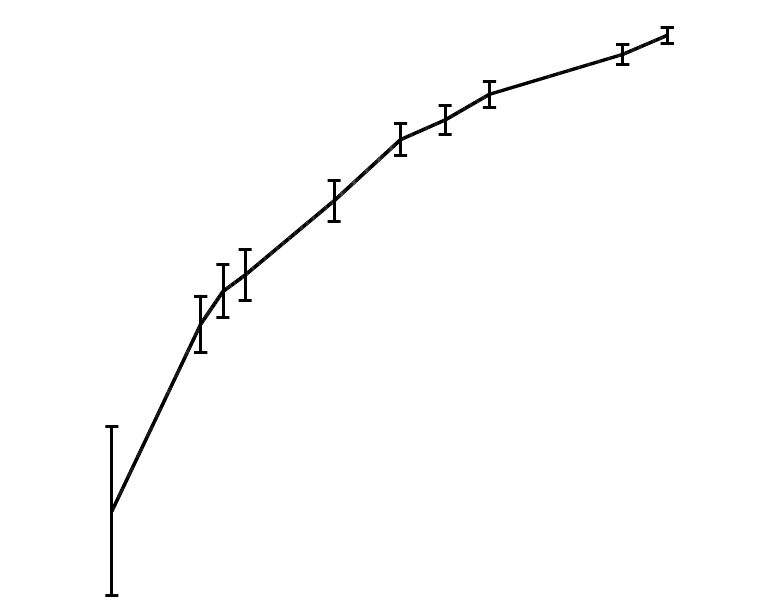
\includegraphics[width=6cm]{img/chap1/reibman1}};
\draw (-7,0) rectangle (0,5.51);
\draw (-7,0.1) -- (-7,0) node[anchor=north] {1};
\draw (-6,0.1) -- (-6,0) node[anchor=north] {1,5};
\draw (-5,0.1) -- (-5,0) node[anchor=north] {2};
\draw (-4,0.1) -- (-4,0) node[anchor=north] {2,5};
\draw (-3,0.1) -- (-3,0) node[anchor=north] {3};
\draw (-2,0.1) -- (-2,0) node[anchor=north] {3,5};
\draw (-1,0.1) -- (-1,0) node[anchor=north] {4};
\draw (0,0.1) -- (0,0) node[anchor=north] {4,5};
\draw (-6.9,1.83) -- (-7,1.83) node[anchor=east] {-5};
\draw (-6.9,3.67) -- (-7,3.67) node[anchor=east] {0};
\draw (-6.9,5.51) -- (-7,5.51) node[anchor=east] {5};
\node[below=0.3cm] at (-3.5,0) {Facteur de l'algorithme};
\node[rotate=90] at (-7.7,2.5) {Qualité subjective relative};
% \end{tikzpicture}\end{tikzpicture}}
	\subfloat[Pour une seule image\label{reibman2}.]{\begin{tikzpicture}[scale=0.853]% \begin{tikzpicture}[scale=0.85]
\node at (-3.5,2.75) {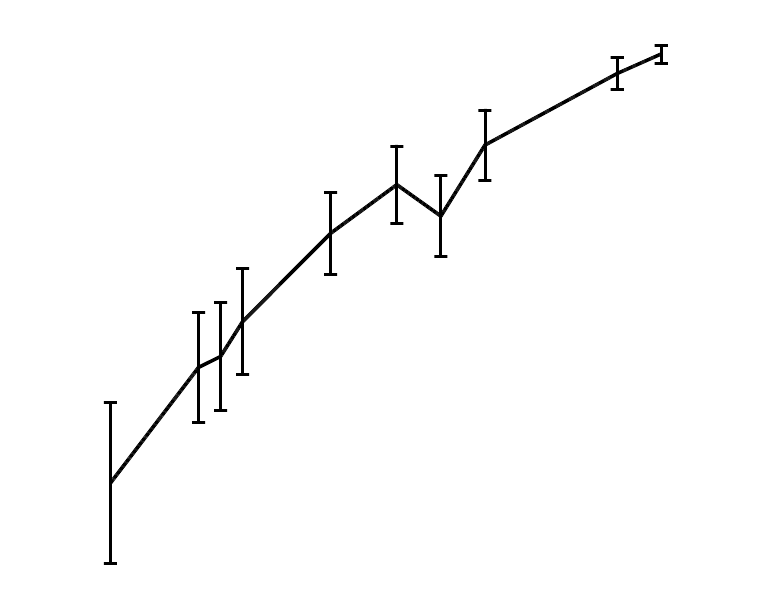
\includegraphics[width=6cm]{img/chap1/reibman2}};
\draw (-7,0) rectangle (0,5.51);
\draw (-7,0.1) -- (-7,0) node[anchor=north] {1};
\draw (-6,0.1) -- (-6,0) node[anchor=north] {1,5};
\draw (-5,0.1) -- (-5,0) node[anchor=north] {2};
\draw (-4,0.1) -- (-4,0) node[anchor=north] {2,5};
\draw (-3,0.1) -- (-3,0) node[anchor=north] {3};
\draw (-2,0.1) -- (-2,0) node[anchor=north] {3,5};
\draw (-1,0.1) -- (-1,0) node[anchor=north] {4};
\draw (0,0.1) -- (0,0) node[anchor=north] {4,5};
\draw (-6.9,0) -- (-7,0) node[anchor=east] {-12};
\draw (-6.9,0.56) -- (-7,0.56) node[anchor=east] {-10};
\draw (-6.9,1.1) -- (-7,1.1) node[anchor=east] {-8};
\draw (-6.9,1.65) -- (-7,1.65) node[anchor=east] {-6};
\draw (-6.9,2.2) -- (-7,2.2) node[anchor=east] {-4};
\draw (-6.9,2.76) -- (-7,2.76) node[anchor=east] {-2};
\draw (-6.9,3.31) -- (-7,3.31) node[anchor=east] {0};
\draw (-6.9,3.87) -- (-7,3.87) node[anchor=east] {2};
\draw (-6.9,4.42) -- (-7,4.42) node[anchor=east] {4};
\draw (-6.9,4.97) -- (-7,4.97) node[anchor=east] {6};
\draw (-6.9,5.51) -- (-7,5.51) node[anchor=east] {8};
\node[below=0.3cm] at (-3.5,0) {Facteur de l'algorithme};
\node[rotate=90] at (-8,2.5) {Qualité subjective relative};
% \end{tikzpicture}\end{tikzpicture}}\\
	\caption{Qualité relative en fonction du paramètre de l'algorithme.}
	\label{fig:reibmanVpqm2006}
\end{figure}

Il existe d'autres modèles de comparaison par paires~\cite{scheffe-jasa,kendall-biometrics,morrissey-josa}. Handley~\cite{handley-pics2001} montre la supériorité du modèle de Bradley--Terry face à la loi du jugement comparatif de Thurstone--Mosteller~\cite{thurstone-psychometrika,mosteller-psychometrika1, mosteller-psychometrika2}, très utilisée par ailleurs~\cite{imberty-rsa,bradlow-jasa}. L'avantage principal du modèle de Bradley--Terry est son efficacité dans le cas où le nombre de comparaisons par paires n'est pas le même pour toutes les images. Cependant, il existe deux importantes restrictions à son usage. La première est que l'ensemble de séquences ne doit pas être décomposables en deux sous-ensembles tels qu'aucune comparaison n'ait été effectuée entre eux. La deuxième est que ces deux sous-ensembles ne doivent pas être tels que toutes les séquences d'un sous-ensemble soient toujours préférées à toutes celles de l'autre sous-ensemble.


\section{Applications en télévision haute définition} \label{tests:TVHD}
Les sections précédentes présentaient des outils en grande partie développés spécifiquement pour la télévision standard. Dans le cadre de leur adaptation à la télévision haute définition, nous devons répondre aux questions suivantes :
\begin{itemize}
\item quelles sont les différences fondamentales entre TVSD et TVHD en termes de conditions de tests ?
\item ces différences ont-elles des conséquences sur les méthodologies déjà existantes et d'autres méthodologies sont-elles à développer ?
\item existe-t-il des expérimentations ayant évalué la qualité visuelle de la TVHD ?
\end{itemize}

Cette section détaille les différences entre TVSD et TVHD qui ont le plus d'influence sur le jugement d'un observateur. Puis nous présenterons trois expérimentations, réalisées par des institutions internationales, sur l'impact de différents facteurs de la TVHD sur la qualité.


\subsection{Que change la télévision haute définition ?} \label{ssec:Que_change_la_télévision_haute_définition}
La télévision haute définition est considérée comme un pas en avant en termes de qualité visuelle. Deux facteurs principaux sont en cause. D'un coté, la plus grande immersion dans l'action est possible grâce au changement de résolution intrinsèque de 720\texttimes576 à 1920\texttimes1080, au passage du format 4$:$3 au format 16$:$9 et plus accessoirement au passage d'un pixel de format 10/9 à un pixel carré. D'un autre côté, l'arrivée à maturité de technologies d'affichage sur écrans plats et de stockage de grande capacité permettent la réalisation technique d'études amorcées au début des années 1980~\cite{fujio-futureHDTV,mitsuhashi-scanning,yuyama-largescreeneffects}. Nous détaillons ici les raisons techniques et psychophysiques du gain en qualité constaté.

\subsubsection{Une qualité accrue par un champ visuel élargi}
Contrairement à la voix et à l'écrit, l'image permet la réception directe d'une grande quantité d'information. À l'époque de sa mise en place, la TVSD devait faire face à des contraintes techniques importantes, notamment au niveau des débits de transmission et des afficheurs. C'est la raison pour laquelle l'image fournie avait un impact visuel réduit sur l'observateur car les technologies ne pouvaient exploiter tout le potentiel des fonctions psychophysiques du système visuel humain. Les sensations et l'émotion ressenties étaient pauvres.

Pour atteindre un plus grand impact psychologique, comme peut le faire le cinéma par exemple, il faut faire converger la zone d'image avec le champ visuel de l'observateur. Cela permet de réduire la sensation de présence de l'appareil de restitution, et de donner de la profondeur et du naturel à l'image. Un tel effet psychologique apparait pour un angle visuel de 20 à 30 degrés dans la direction horizontale. Parallèlement, deux impératifs sont à respecter. Tout d'abord, la structure en lignes ne doit pas être visible. La continuité spatiale de l'image doit donc être assurée. Dans cette optique, la valeur retenue dans le cadre de la TVSD est un ratio entre distance d'observation et hauteur de l'écran égal à six. Dans le cadre de la TVHD, ce ratio est à recalculer. Le second impératif est que le mouvement doit rester fluide, tout en considérant que le système visuel humain ne peut pas suivre un mouvement trop rapide. Le tableau~\ref{tab:DistanceLigneAngle} donne le nombre minimal de lignes que doit contenir une image pour obtenir l'angle visuel donné dans la direction horizontale, en se situant à la distance $O$ de l'écran, le tout sans pouvoir différencier le fait que l'image est constituée de lignes~\cite{fujio-futureHDTV}. La distance $O$ est donnée comme un multiple de la hauteur $H$ de l'écran. Très tôt, des tests ont permis de déterminer la distance idéale pour regarder une image animée sans générer de fatigue~\cite{fujio-futureHDTV,mitsuhashi-scanning,yuyama-largescreeneffects}. Celle-ci est de quatre fois la hauteur de l'écran pour des scènes contenant du mouvement rapide et de trois fois la hauteur de l'écran pour les autres scènes. Ainsi d'après le tableau~\ref{tab:DistanceLigneAngle}, il faut une image d'environ 1200 lignes. C'est un peu plus que le double de celle d'une image de TVSD.

\begin{table}[htbp]
\centering
\begin{tabular}[c]{ccccccc}\toprule
\strong{distance} $O$					& 7,2$H$	& 4$H$		& 3,3$H$	& 3$H$		& 2,5$H$	& 2$H$	\\\midrule
\strong{angle visuel $\Theta$ (degré)}	& 10,7		& 23,5		& 28,3		& 31,0		& 36,9		& 45,2	\\\midrule
\strong{nombre de lignes} $N_L$		& 525		& 940		& 1125		& 1240		& 1480		& 1840	\\\bottomrule
\end{tabular}
\caption{Nombre de lignes $N_L$ requis pour obtenir l'angle visuel $\Theta$ dans la direction horizontale, en se situant à la distance $O$ de l'écran et sans distinguer les lignes.}
\label{tab:DistanceLigneAngle}
\end{table}

Pour augmenter l'impact psychologique de la télévision, la solution consiste donc à agrandir l'image, afin de pouvoir bénéficier d'un angle visuel d'environ 30 degrés en se plaçant à environ trois fois fois la hauteur de l'écran. C'est ainsi que se justifie les dimensions de la télévision haute définition. Plus récemment, d'autres études sont venues confirmer ces valeurs~\cite{svt-assesstudy} et VQEG les utilise dans ses expérimentations~\cite{vqeg-hdtvtestplan}. La proportion de champ visuel excité par l'image passe ainsi de 4\% à 20\% comme l'illustre la figure~\ref{fig:champVisuelHD}. Cependant, une telle augmentation a des conséquences sur l'observateur. Souvent en mouvement, la zone d'intérêt est plus importante, et demande donc une plus grande attention. Les effets de cette immersion sur la perception de l'image nécessitent des études différentes de celles réalisées pour la télévision standard.

\begin{figure}[htbp]
  \centering
  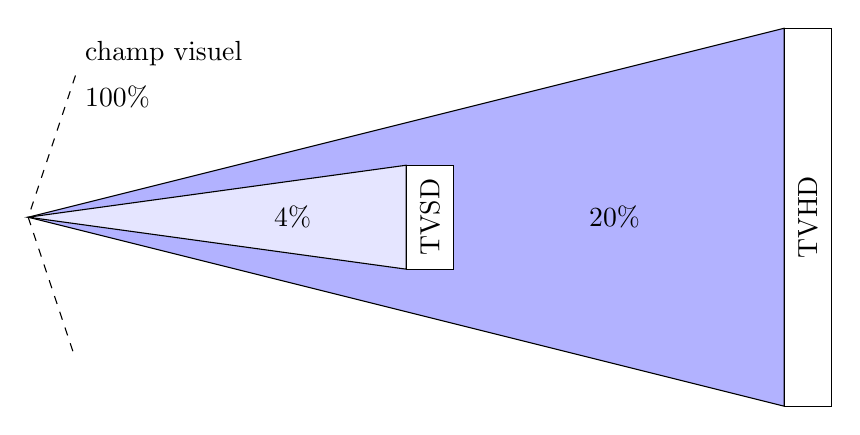
\begin{tikzpicture}[text centered, scale=1.2]\draw[dashed] (0.5,1.5) node[above right] {champ visuel} node[below right] {100\%}-- (0,0) -- (0.5,-1.5);
\filldraw[fill=blue!30] (0,0) node[right=7cm] {20\%} -- (8,2) -- (8,-2) -- cycle;
\filldraw[fill=blue!10] (0,0) node[right=3cm] {4\%} -- (4,0.55) -- (4,-0.55) -- cycle;
\draw (8,2) rectangle node[rotate=90] {TVHD} (8.5,-2);
\filldraw[fill=white] (4,0.55) rectangle node[rotate=90] {TVSD} (4.5,-0.55);
\end{tikzpicture}
  \caption{Proportions de champ visuel excité par les formats TVSD et TVHD.}
  \label{fig:champVisuelHD}
\end{figure}


\subsubsection{Un manque de matériel disponible}
La TVHD manque encore de matériel spécifique tant en production qu'en test ou en visualisation. De même, les protocoles de tests subjectifs sont encore à spécifier, VQEG y consacre d'ailleurs une partie de ses activités~\cite{vqeg-hdtvtestplan}. Les différences avec la TVSD y sont peu marquées à l'heure actuelle, et elles concernent surtout les spécifications de l'environnement de test. Parallèlement, la réalisation de ces tests pour les laboratoires nécessite de pouvoir disposer de vidéos au format TVHD, si possible libres de droits. Actuellement, quelques séquences sont disponibles mais le format est encore minoritairement utilisé. Certains contenus, comme les évènements sportifs, sont particulièrement difficiles à obtenir, alors que leur intérêt est primordial dans l'optique de l'établissement d'un large service de TVHD.

Ce manque rend difficile les études sur télévision haute définition et notamment l'évaluation subjective de la qualité visuelle. Cela explique donc le peu d'études spécifiques à ce format dans la littérature, et particulièrement dans le monde universitaire. Pourtant, l'enjeu scientifique et technique qu'est la mise en place d'un système de TVHD est important.


\subsection{Expériences sur l'impact de la technologie d'affichage} \label{ssec:itu}
En 2005, l'ITU a publié les résultats d'une étude effectuée par l'\emph{Association of radio industries and businesses} japonaise~\cite{itu-crtlcd}. Le but était de comparer les écrans de type CRT aux écrans de type LCD. La méthodologie d'évaluation utilisée était une méthodologie de comparaison simultanée avec une échelle à sept niveaux. Ici, seuls des experts ont pris part aux tests mis en place selon la recommandation spécifiquement dédiée à la TVHD, l'ITU-R BT.710-4~\cite{itu-bt710-4}. Les deux écrans testés étaient un CRT d'usage professionnel de 24 pouces et de résolution 1920\texttimes1080 et un LCD grand public de 23 pouces et de résolution 1280\texttimes768. Les séquences étaient au nombre de 30.

Les résultats montrent une légère préférence pour le CRT. Les meilleurs scores de qualité en sa faveur sont obtenus avec des séquences contenant soit du mouvement, soit des zones sombres. Or, le flou de mouvement et le rendu des zones sombres sont deux des défauts connus du LCD. De plus, la différence de résolution était en défaveur du LCD et était clairement perçue par les experts. Par contre, les couleurs sont mieux appréciées sur le LCD, ainsi que le rendu des zones claires.

Bien sûr, cette étude ne permet pas de conclure catégoriquement sur les différences de qualité entre CRT et LCD. Néanmoins, elle souligne la nécessité d'étudier les différences de technologie, à l'heure où le CRT cède sa place aux technologies à écrans plats.


\subsection{Expériences sur l'impact du format d'image dans un contexte de codage \avc} \label{ssec:ebu}
\begin{wrapfigure}{r}{0.3\linewidth}
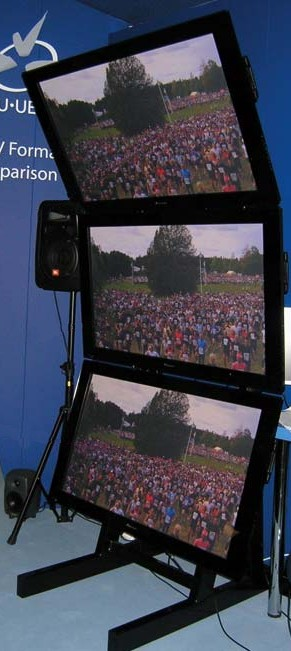
\includegraphics[width=1\linewidth]{img/chap1/ebu}
\caption{Montage de visualisation simultanée de trois écrans HD.} % FIXME voir la mise en page une fois le texte fixé
\label{fig:TroisEcransEBU}
\end{wrapfigure}
Lors de l'\emph{International Broadcasting Convention} de septembre 2006, l'EBU a effectué une expérimentation auprès des participants~\cite{hoffmann-ibc2006}. La démonstration, très formelle étant donné le contexte, permettait de comparer les trois formats de TVHD : 720p/50, 1080i/25 et 1080p/50. Le même contenu était projeté simultanément sur trois écrans 1080p. La figure~\ref{fig:TroisEcransEBU} présente le montage permettant cette visualisation simultanée. Le but était de comparer directement la qualité visuelle de la TVHD en mode entrelacé et en mode progressif, et notamment de montrer l'intérêt du 720p. C'est pourquoi celui-ci était placé sur l'écran du centre. Huit personnes pouvaient s'installer simultanément : quatre à une distance de trois fois la hauteur d'un écran et quatre à quatre fois la hauteur d'un écran. Les séquences utilisées ont été fournies par le SVT et l'EBU et codées par le codeur de référence \avc{} à 20, 18, 16, 13, 10, 8 et 6 Mbps. Les contenus aux formats 1080i et 720p étaient issus du format 1080p en subissant respectivement un désentrelacement et un sous-échantillonnage.

Avec les séquences non compressées, les observateurs percevaient peu de différences entre les trois formats, même à une distance de visualisation de trois fois la hauteur de l'écran. Par contre, suivant la distance d'observation et le contenu, les dégradations apparaissaient avec la compression. Le format 720p donnait une meilleure qualité que le format 1080i pour toutes les séquences et à tous les débits. De plus, plus le débit diminuait, plus les différences entre les formats 720p et 1080i étaient marquées. Enfin, en comparant les formats 720p et 1080p, les observateurs les évaluaient de manière équivalente à haut débit. Par contre, le format 720p était plus apprécié que le format 1080p à bas débit. L'EBU explique cela par le fait que le format 1080p surcharge le codeur en information. Ainsi, suivant le contenu, cette surcharge devient le facteur dominant dans la dégradation de la qualité.

Cette étude, bien que peu formalisée, est intéressante, non seulement pour l'originalité de son installation, mais également pour ses conclusions. Ce n'est pas la première fois que l'EBU affirme la supériorité du format 720p sur le format 1080i et le conseille en production~\cite{wood-hd4u,laven-hdtvWars}. Néanmoins, le marché européen se dirige plutôt vers le 1080i, ce qui risque d'amplifier la problématique de l'évaluation de la qualité. Enfin, si le format 1080p semble montrer de bonnes performances à très haut débit, il nécessite encore des études plus approfondies.


\subsection{Expériences sur l'impact des formats d'image et d'écran dans un contexte de codage MPEG-2} \label{ssec:svt}
Un rapport sur l'évaluation de qualité de séquences HD et SD a été publié en 2002 par la chaine de télévision suédoise SVT~\cite{svt-assesstudy}. Trois études y sont décrites. La première évalue la TVSD sur des écrans de résolution 852\texttimes480. La deuxième s'intéresse aux différences entre la TVSD et la TVHD 720p sur ces mêmes écrans et sur des écrans de résolution 1366\texttimes768 pixels. Enfin, la troisième décrit les différences entre la TVSD et la TVHD 1080i sur des écrans de résolution 1366\texttimes768. Cette dernière étude porte également sur le gain en codage MPEG-2 à l'utilisation du format 720p à la place du format 1080i. Les paramètres utilisés sont le débit, le contenu des séquences et la distance d'observation. Les séquences pour chaque format ont été codées à six débits différents. Pour le format TVHD, les débits utilisés sont : environ 600 megabits par seconde (Mbps) pour la version non compressée, puis 22, 19, 16, 13 et 10 Mbps. Pour le format TVSD, les débits sont : environ 120 Mbps pour la version non compressée, puis 13, 10, 8, 6 et 4 Mbps. Les tests ont été réalisés avec une distance d'observation variant de quatre à six fois la hauteur de l'écran. Les séquences utilisées ont été créées pour ces tests et sont depuis à la disposition de la communauté scientifique. Deux ensembles d'observateurs les ont évalué. Le premier était composé d'experts en qualité vidéo, le second comportait des personnes non expertes. Les écrans utilisés étaient soit de type PDP \emph{(plasma display panel)} de 42 à 50 pouces, soit des CRT de 17 à 32 pouces. Les experts n'ont visualisé qu'une seule des quatre séquences, mais il s'agissait de celle considérée comme la plus critique. La méthodologie d'évaluation retenue a été le DSCQS, présentée en~\ref{tests:dscqs}. L'échelle des adjectifs qualificatifs a dû être traduite en suédois, à partir des versions déjà existantes. Ceci montre que les termes utilisés sont ressentis différemment suivant les cultures et qu'établir une échelle de qualité demande notamment de prendre en compte les spécificités culturelles de la population composant un panel d'observateur. Cela montre également que ce panel doit avoir une certaine cohérence vis-à-vis de la manière dont les tests dont réalisés.

Le premier enseignement de ce rapport est que les résultats des non experts sont confirmés par ceux des experts. C'est pourquoi nous nous contenterons de l'analyse plus critique de ces derniers. La figure~\ref{fig:svtAssessStudy} présente un exemple de résultats obtenus sur deux séquences par les formats TVSD et TVHD 1080i. Les experts considèrent que la TVSD à 4 Mbps sur un écran de 50 pouces de résolution 1366\texttimes768 produit des images de qualité non acceptable. Même sans compression, l'adaptation de l'image à une résolution plus élevée engendre des dégradations trop visibles pour une utilisation courante. Cela suggère donc que la TVSD ne doit pas être utilisée à des résolutions supérieures à celles qu'elle connait déjà. Par contre, le format 1080i est celui attendue pour un écran de 50 pouces. Cependant, dès 22 Mbps, des distorsions deviennent perceptibles. En descendant à un débit de 10 Mbps, le format 720p est bon, même si quelques dégradations sont visibles. La TVSD n'est pas assez bon et le format 1080i est clairement jugé non acceptable à un tel débit en MPEG-2. L'étude voit en cette dernière comparaison la preuve que le mode progressif est meilleur en terme de codage. Ce gain pourrait permettre de transmettre à la fois un flux TVHD et un flux TVSD. Enfin, les observateurs ont considéré comme idéale une distance d'observation de 4 fois la hauteur d'écran.

\begin{figure}[htbp]
	\centering
	\subfloat[Séquence \emph{Knightshields}.]{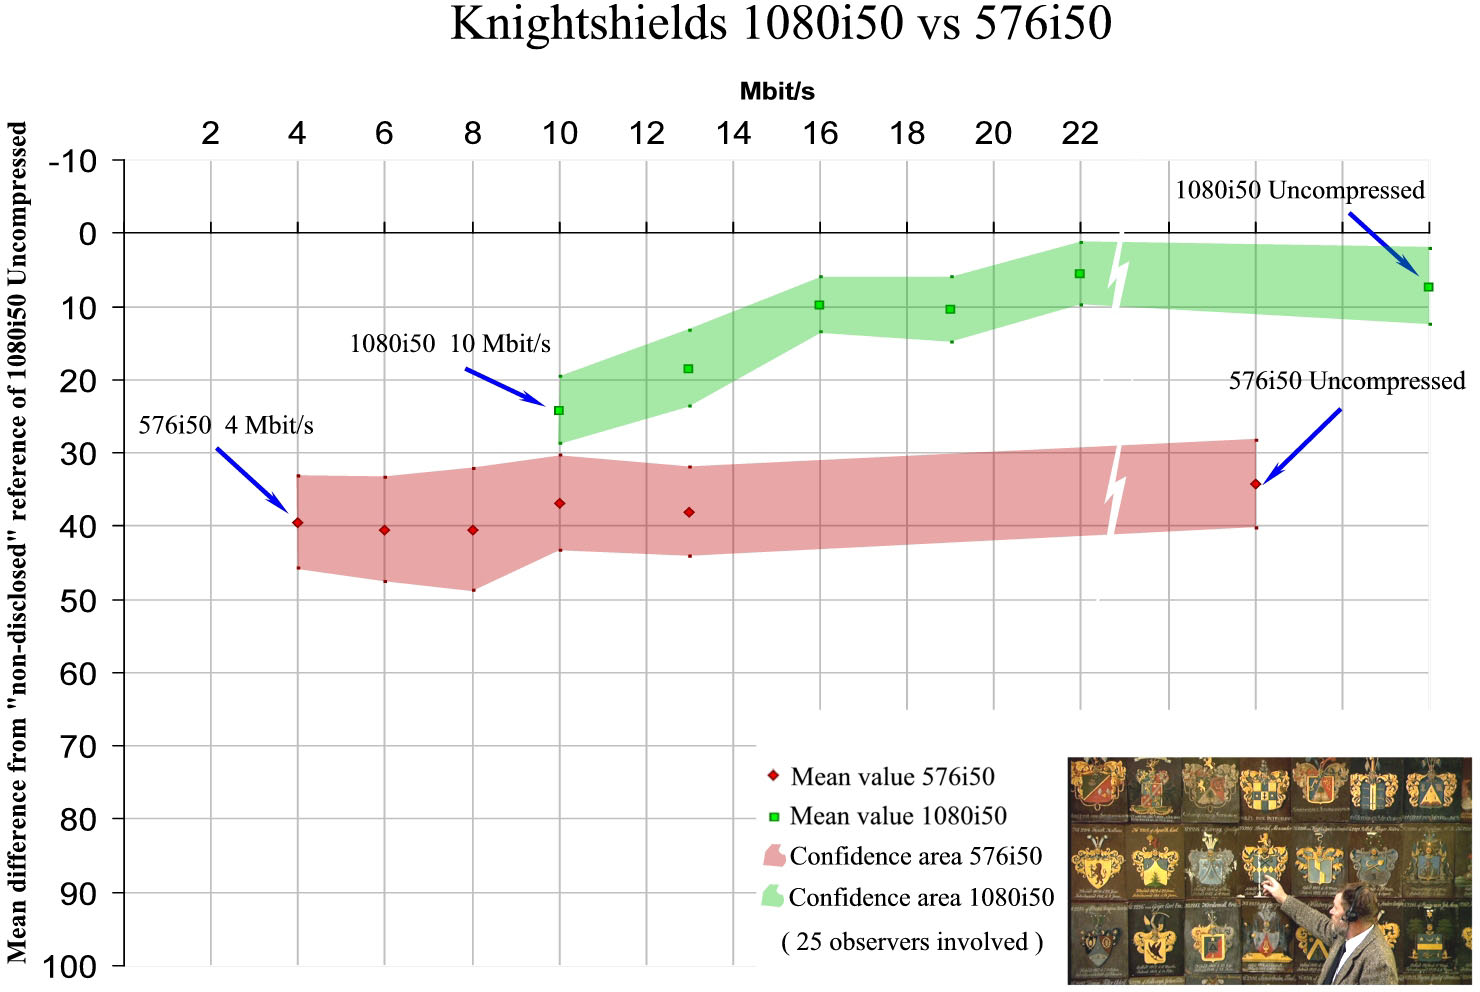
\includegraphics[width=0.48\linewidth]{img/chap1/svt-shields}}\hfill
	\subfloat[Séquence \emph{Stockholm Pan}.]{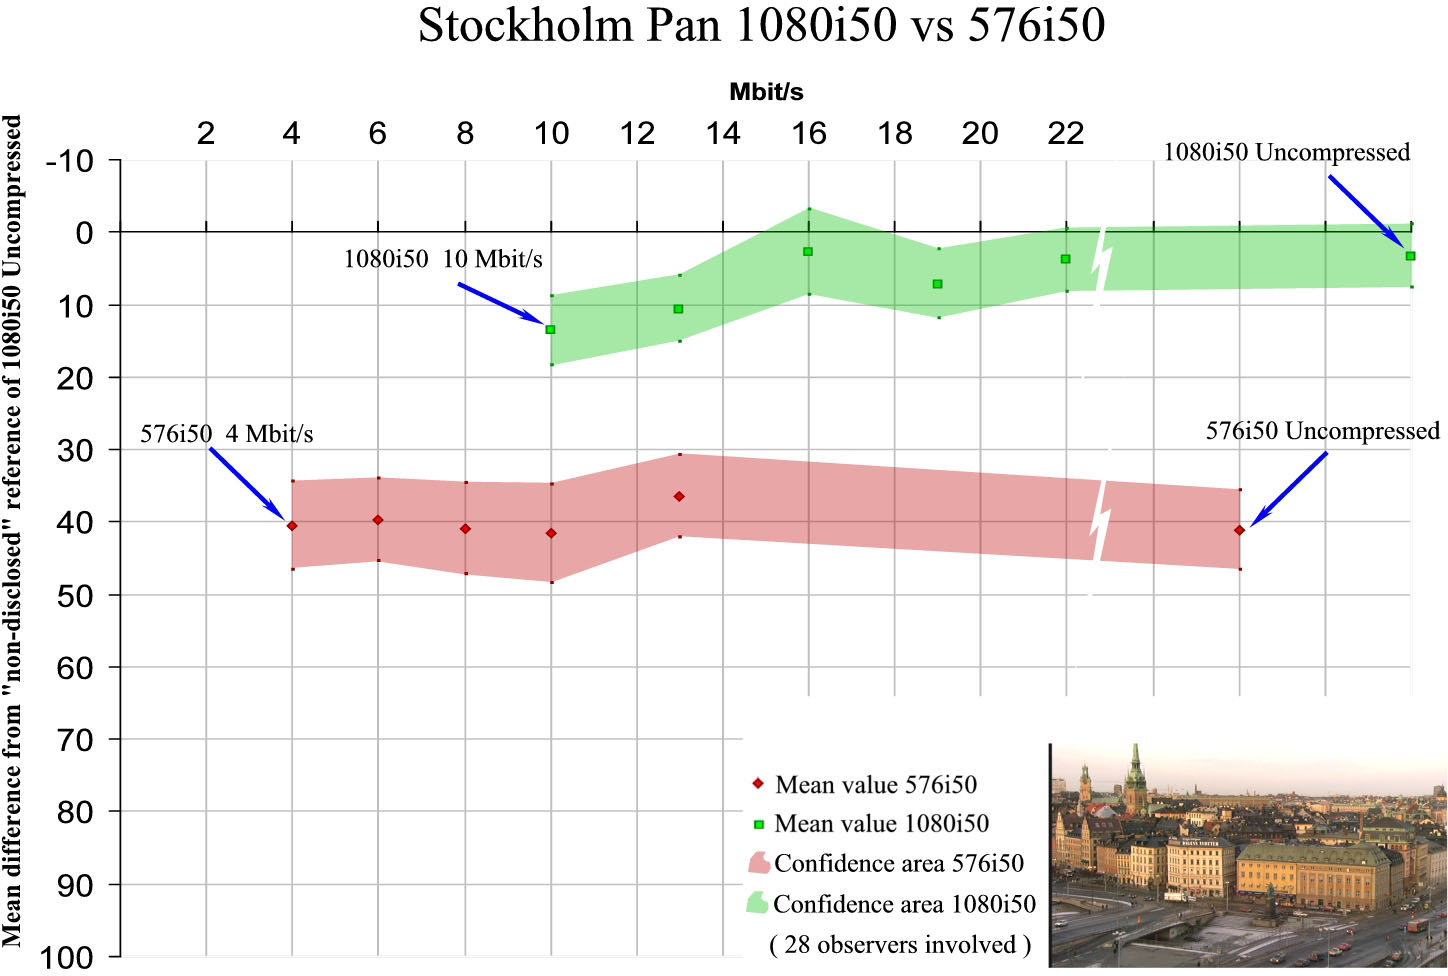
\includegraphics[width=0.48\linewidth]{img/chap1/svt-stockholm}}\\
	\caption{Exemple de résultats obtenus par SVT~\cite{svt-assesstudy}.}
	\label{fig:svtAssessStudy}
\end{figure}

Ce rapport est intéressant pour l'étude de la transition de la TVSD à la TVHD. Elles montrent les lacunes de la TVSD et le gain en qualité des formats 720p et 1080i sur des écrans de haute résolution. Cependant, aucun des écrans utilisés n'offrait les résolutions natives 1280\texttimes720 ou 1920\texttimes1080. De plus, il n'est pas prévu d'utiliser le codage MPEG-2 à terme pour de la diffusion HD. L'évaluation des performances du codage \avc{} est donc importante à réaliser, et ce sur des résolutions qui seront celles utilisées à plus ou moins long terme, à savoir le format 1080i et le format 1080p.


\subsection{Conclusion}
Dans cette section, nous avons explicité les changements induits par la télévision haute définition. Cela a permis de mettre en évidence le fait que ces changements étaient substantiels et que leurs conséquences sur l'évaluation subjective de la qualité devaient être étudiées en profondeur. Nous avons également présenté quelques applications récentes à la télévision haute définition de méthodologies existantes. Toutes ont été réalisées par des institutions, l'implication du monde universitaire dans ce domaine étant particulièrement faible. Ces études proposaient l'analyse d'un des facteurs nouveaux de la TVHD comme la résolution ou le type d'affichage. Malheureusement, la seule étude à utiliser des écrans de résolution 1920\texttimes1080 a réalisé ses tests dans un environnement non normalisé et de manière très informelle, sans relever de données quantitatives. Il y a donc encore de nombreux paramètres à caractériser, en se plaçant dans les conditions réelles du service futur de la TVHD, à savoir avec un écran plat de résolution 1920\texttimes1080 et un système de codage \avc.


\section{Conclusion}
Ce premier chapitre a introduit certains concepts de la problématique d'évaluation subjective de la qualité visuelle en télévision haute définition. Tout d'abord, nous avons présenté les méthodologies les plus couramment utilisées. Nous avons vu qu'il en existe plusieurs, chacune ayant un objectif particulier. Comme certaines études ont pu le montrer, elles ne sont pas interchangeables. Leur principal défaut est qu'elles concernent en grande partie la TVSD, les spécificités de la TVHD n'ayant pas encore été suffisamment considérées dans la normalisation internationale. Ensuite, nous avons présenté la manière dont les évaluations récoltées sont analysées. Cette étape est fondamentale, à la fois pour la vérification de la cohérence des observateurs, mais également pour la synthèse des données en quelques valeurs numériques significatives. Enfin, nous avons détaillé les différences entre la télévision standard et la télévision haute définition. Celles-ci influent sur la manière dont l'évaluation subjective de la qualité doit être pensée pour la TVHD. Des études sur l'impact de la TVHD sur la perception de la qualité ont également été présentées.

Par leur nombre, ces études montrent le peu d'éléments existant sur l'évaluation subjective de la qualité visuelle spécifique à la TVHD. Pire, aucune des expérimentations évoquées ne se place dans des conditions idéales d'évaluation normalisées de la TVHD telle qu'elle est en cours d'apparition en Europe. D'ailleurs, les recommandations internationales, très utilisées pour la TVSD, ne considèrent pas les évolutions majeures induites par cette transition. Celles-ci sont à la fois d'ordre technique et psychophysique. Le côté psychophysique est introduit par la distance d'observation, fortement réduite en TVHD. Cela entraine un plus grand champ visuel excité, et donc une perception de la qualité et des dégradations profondément modifiée. D'un point de vue technique, l'affichage subit une mutation importante puisque les écrans CRT cèdent irrémédiablement la place aux écrans plats, plus grands, moins encombrants et plus lumineux. Ce changement de technologie d'affichage a évidemment des répercussions sur la perception de l'image par l'observateur et peut engendrer tantôt une perte tantôt un gain en qualité qu'il convient d'estimer.


\ornementChapitre
